\clearpage
\subsection{Utterance-average confidence versus \texttt{avg\_logprob}}\label{subsec:conf-vs-lprob}

\begin{figure}[h!]
 \caption{Per-conversation average WER when evaluating in non-descending order of utterance \texttt{avg\_logprob}}
 \label{fig:average-avg-logprob}
 \centering
 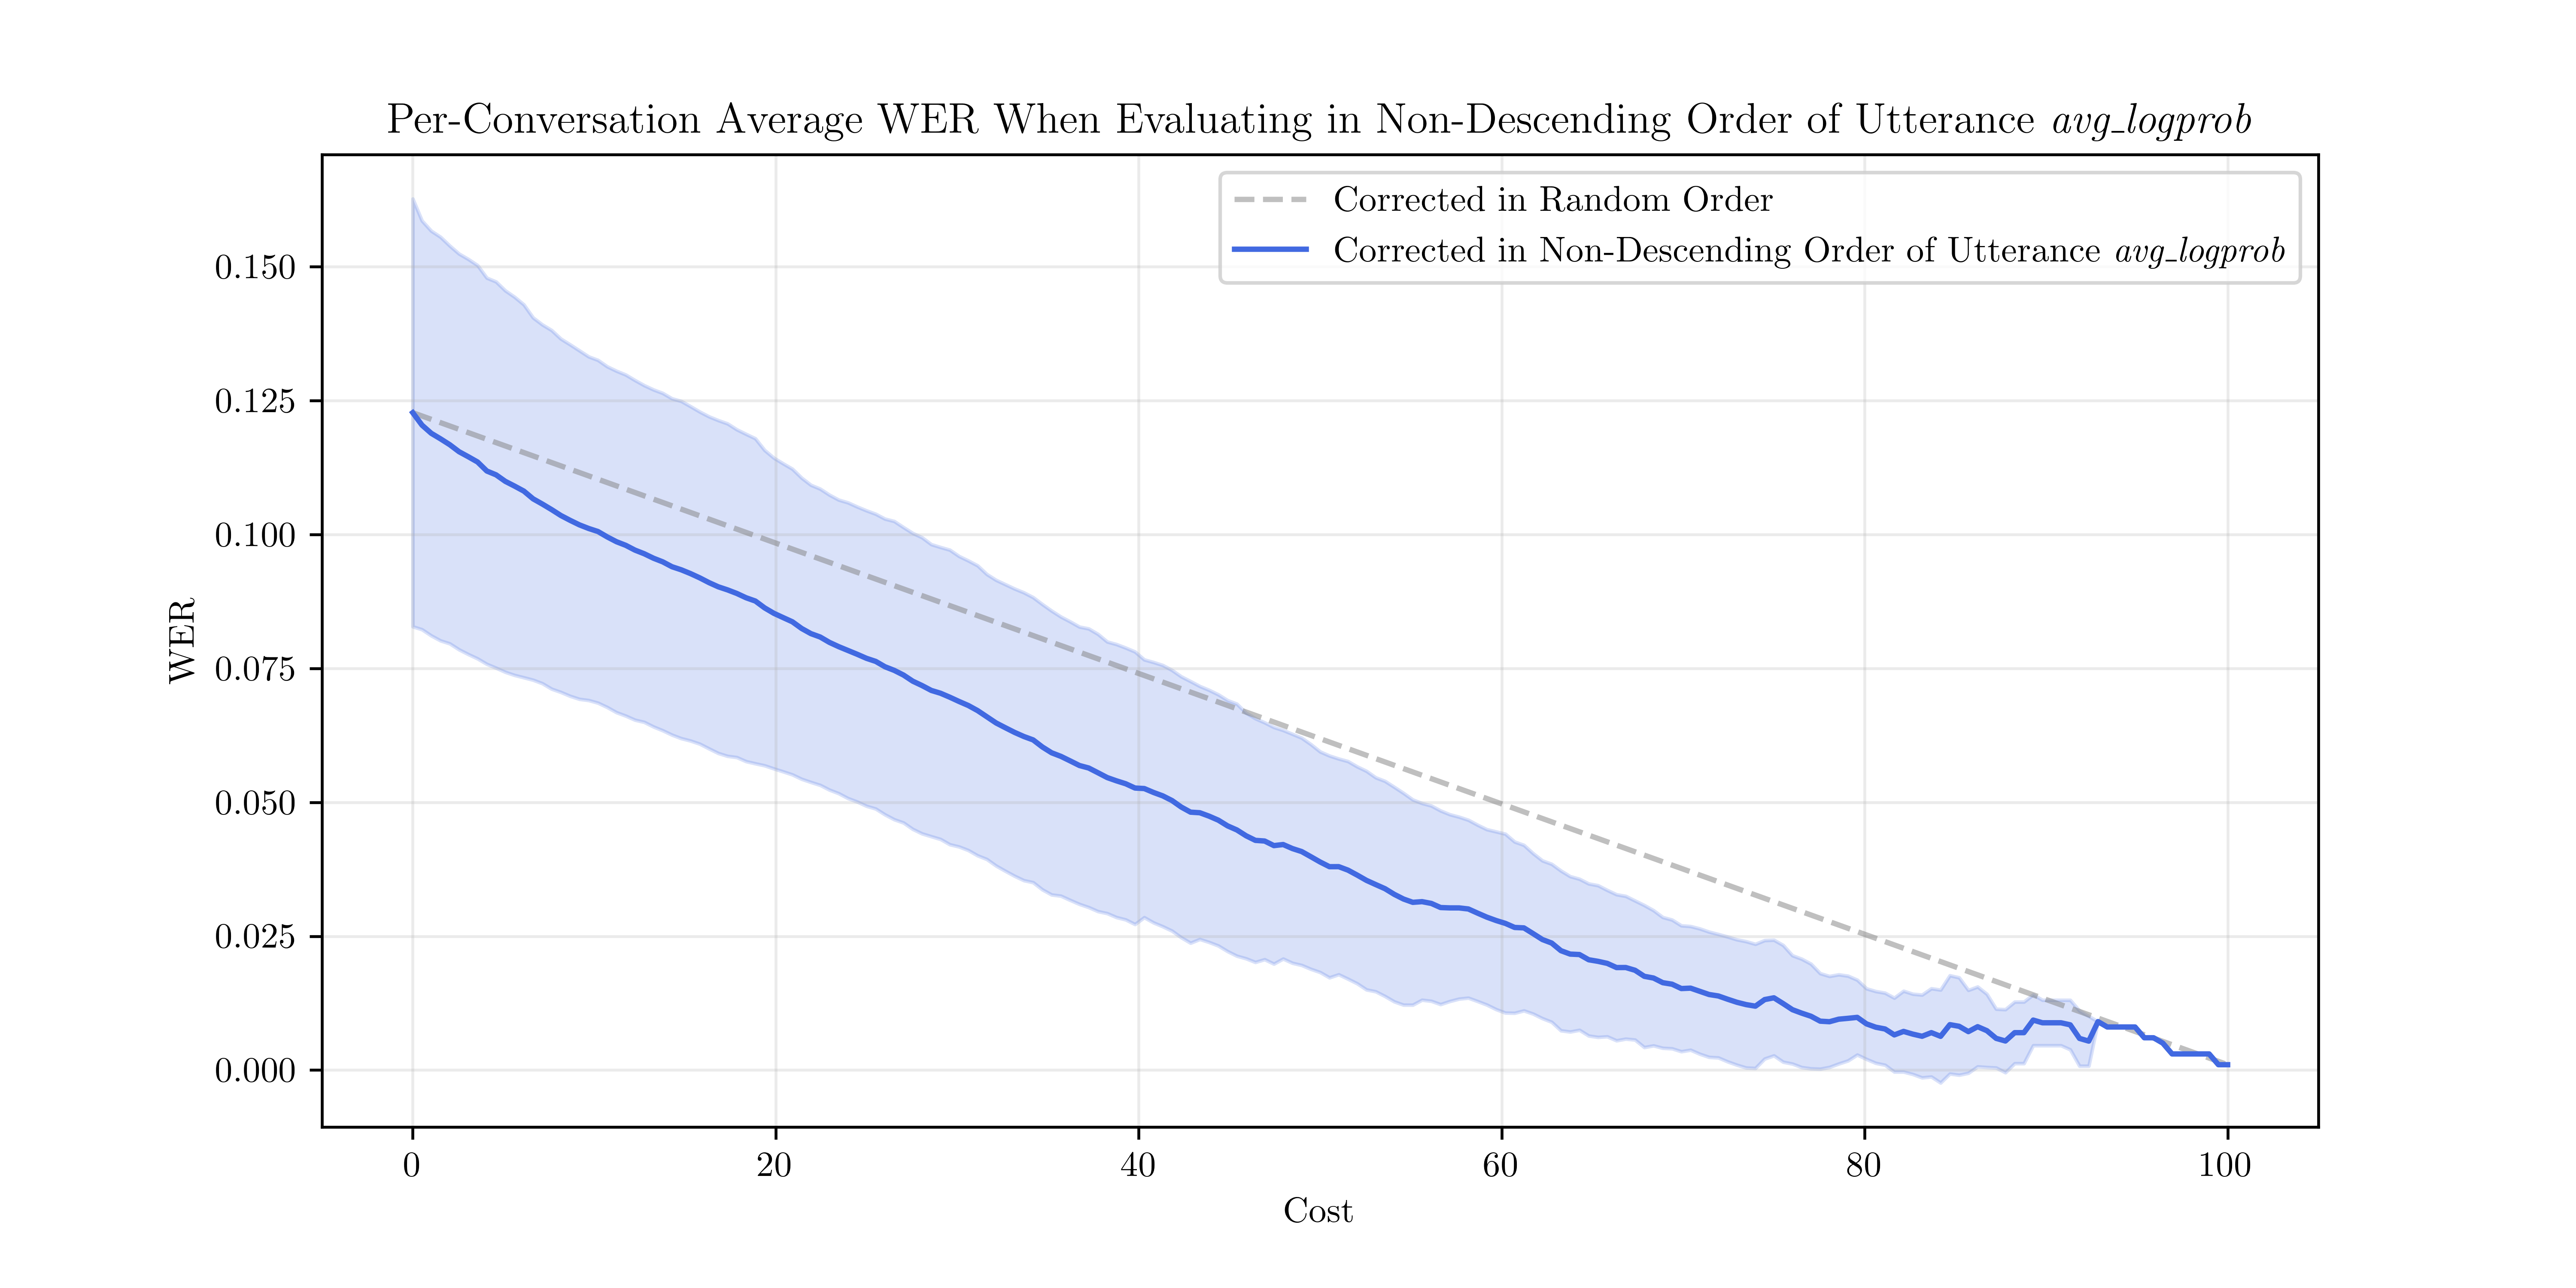
\includegraphics[width=\textwidth]{figures/average-avg-logprob.png}
\end{figure}
\begin{figure}[h!]
 \caption{Per-conversation average WER when evaluating in non-descending order of utterance-average confidence}
 \label{fig:average-uttconf}
 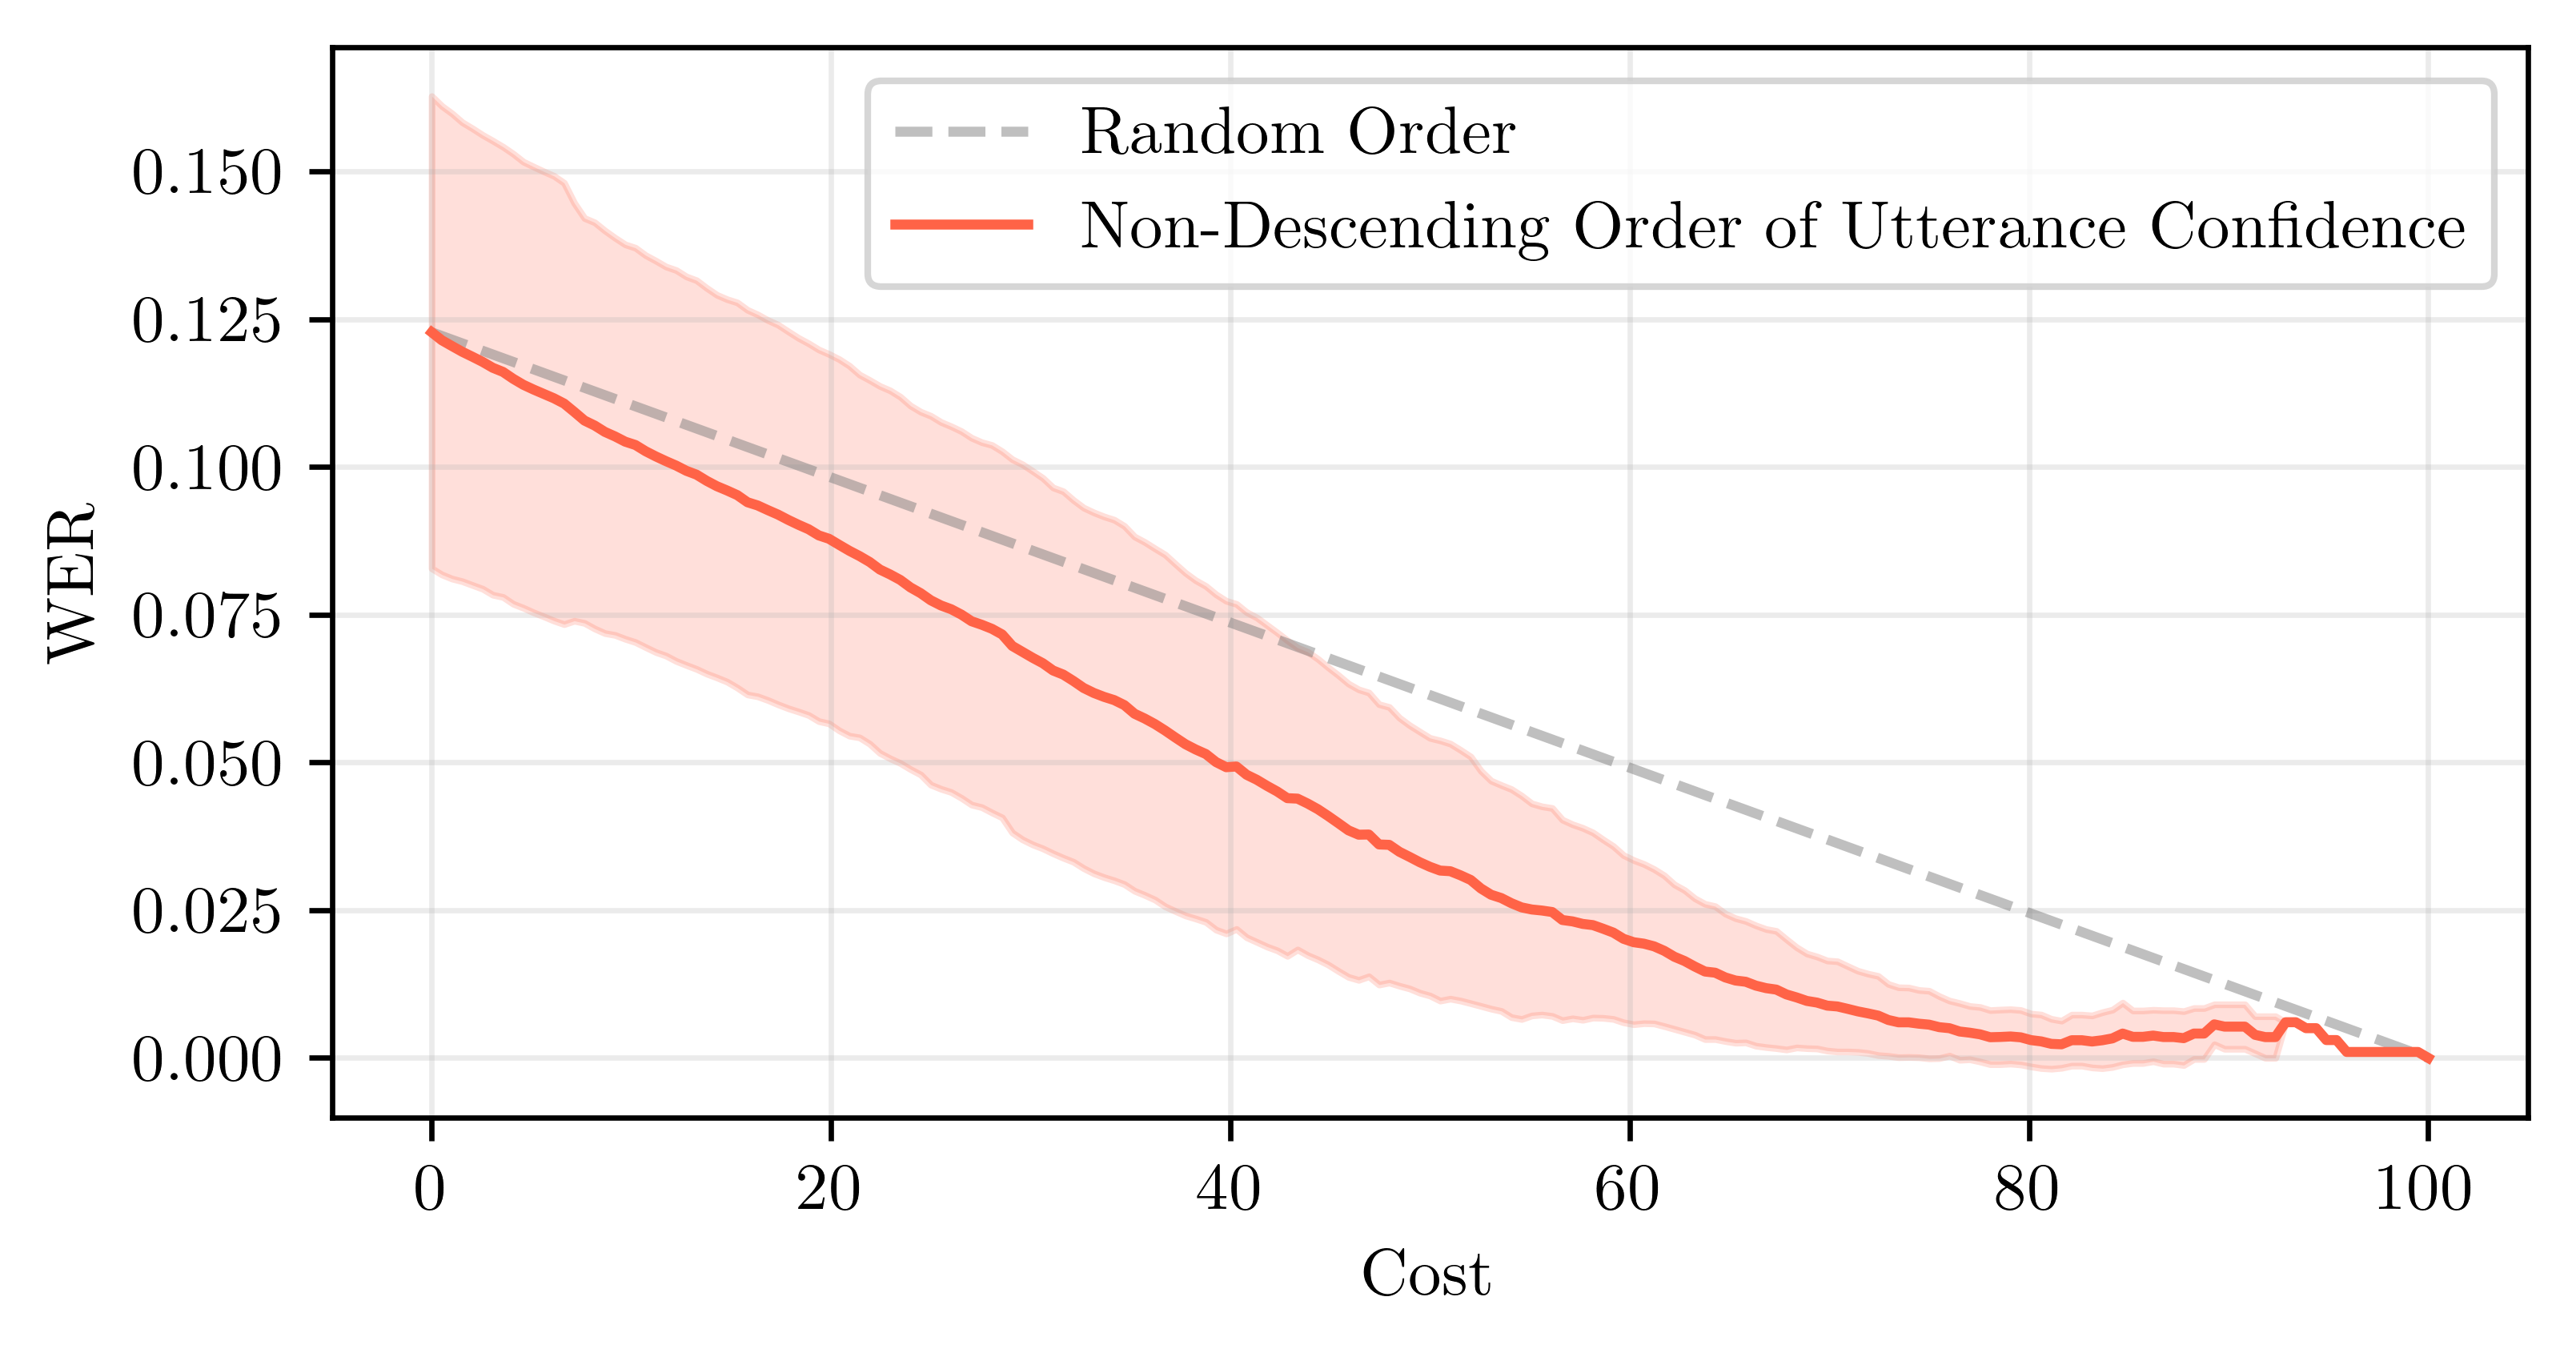
\includegraphics[width=\textwidth]{figures/average-uttconf.png}
 \centering
\end{figure}
\begin{figure}[p]
 \caption{Comparing per-conversation average performance of confidence and \texttt{avg\_logprob}}
 \label{fig:compare-avg-uttconf-vs-lprob}
 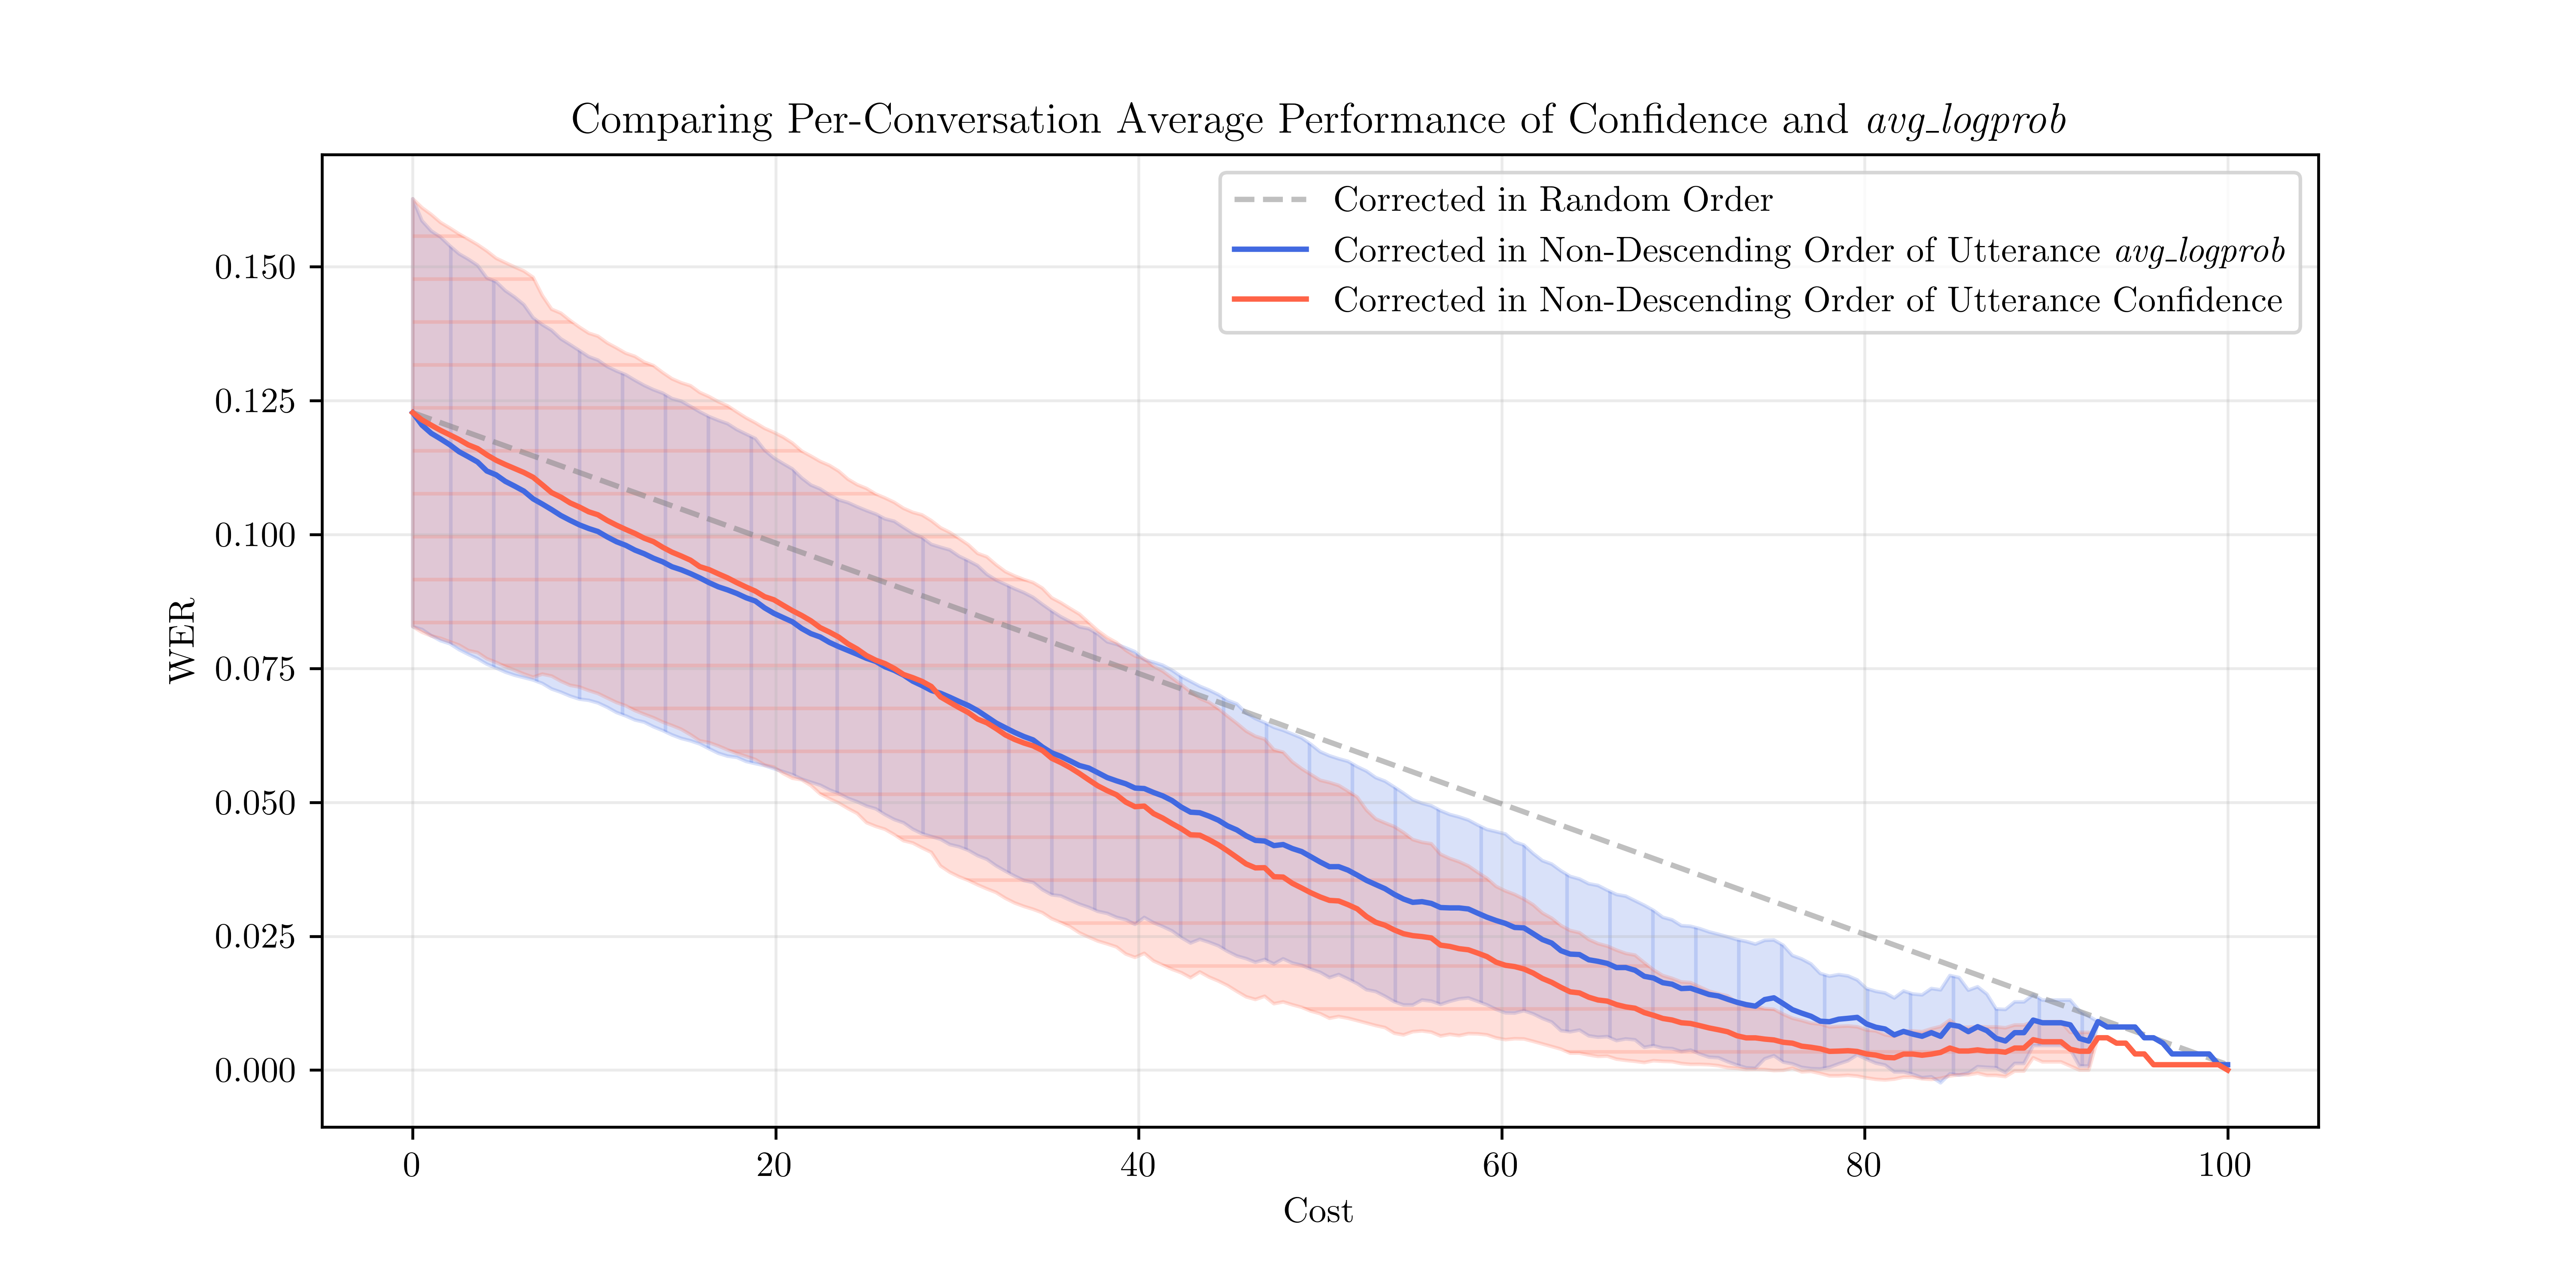
\includegraphics[width=\textwidth]{figures/compare-avg-uttconf-vs-lprob.png}
 \centering
\end{figure}
\begin{figure}[p]
 \caption{Comparing whole-corpus performance of confidence and \texttt{avg\_logprob}}
 \label{fig:corpus-avg-lprob-uttconf}
 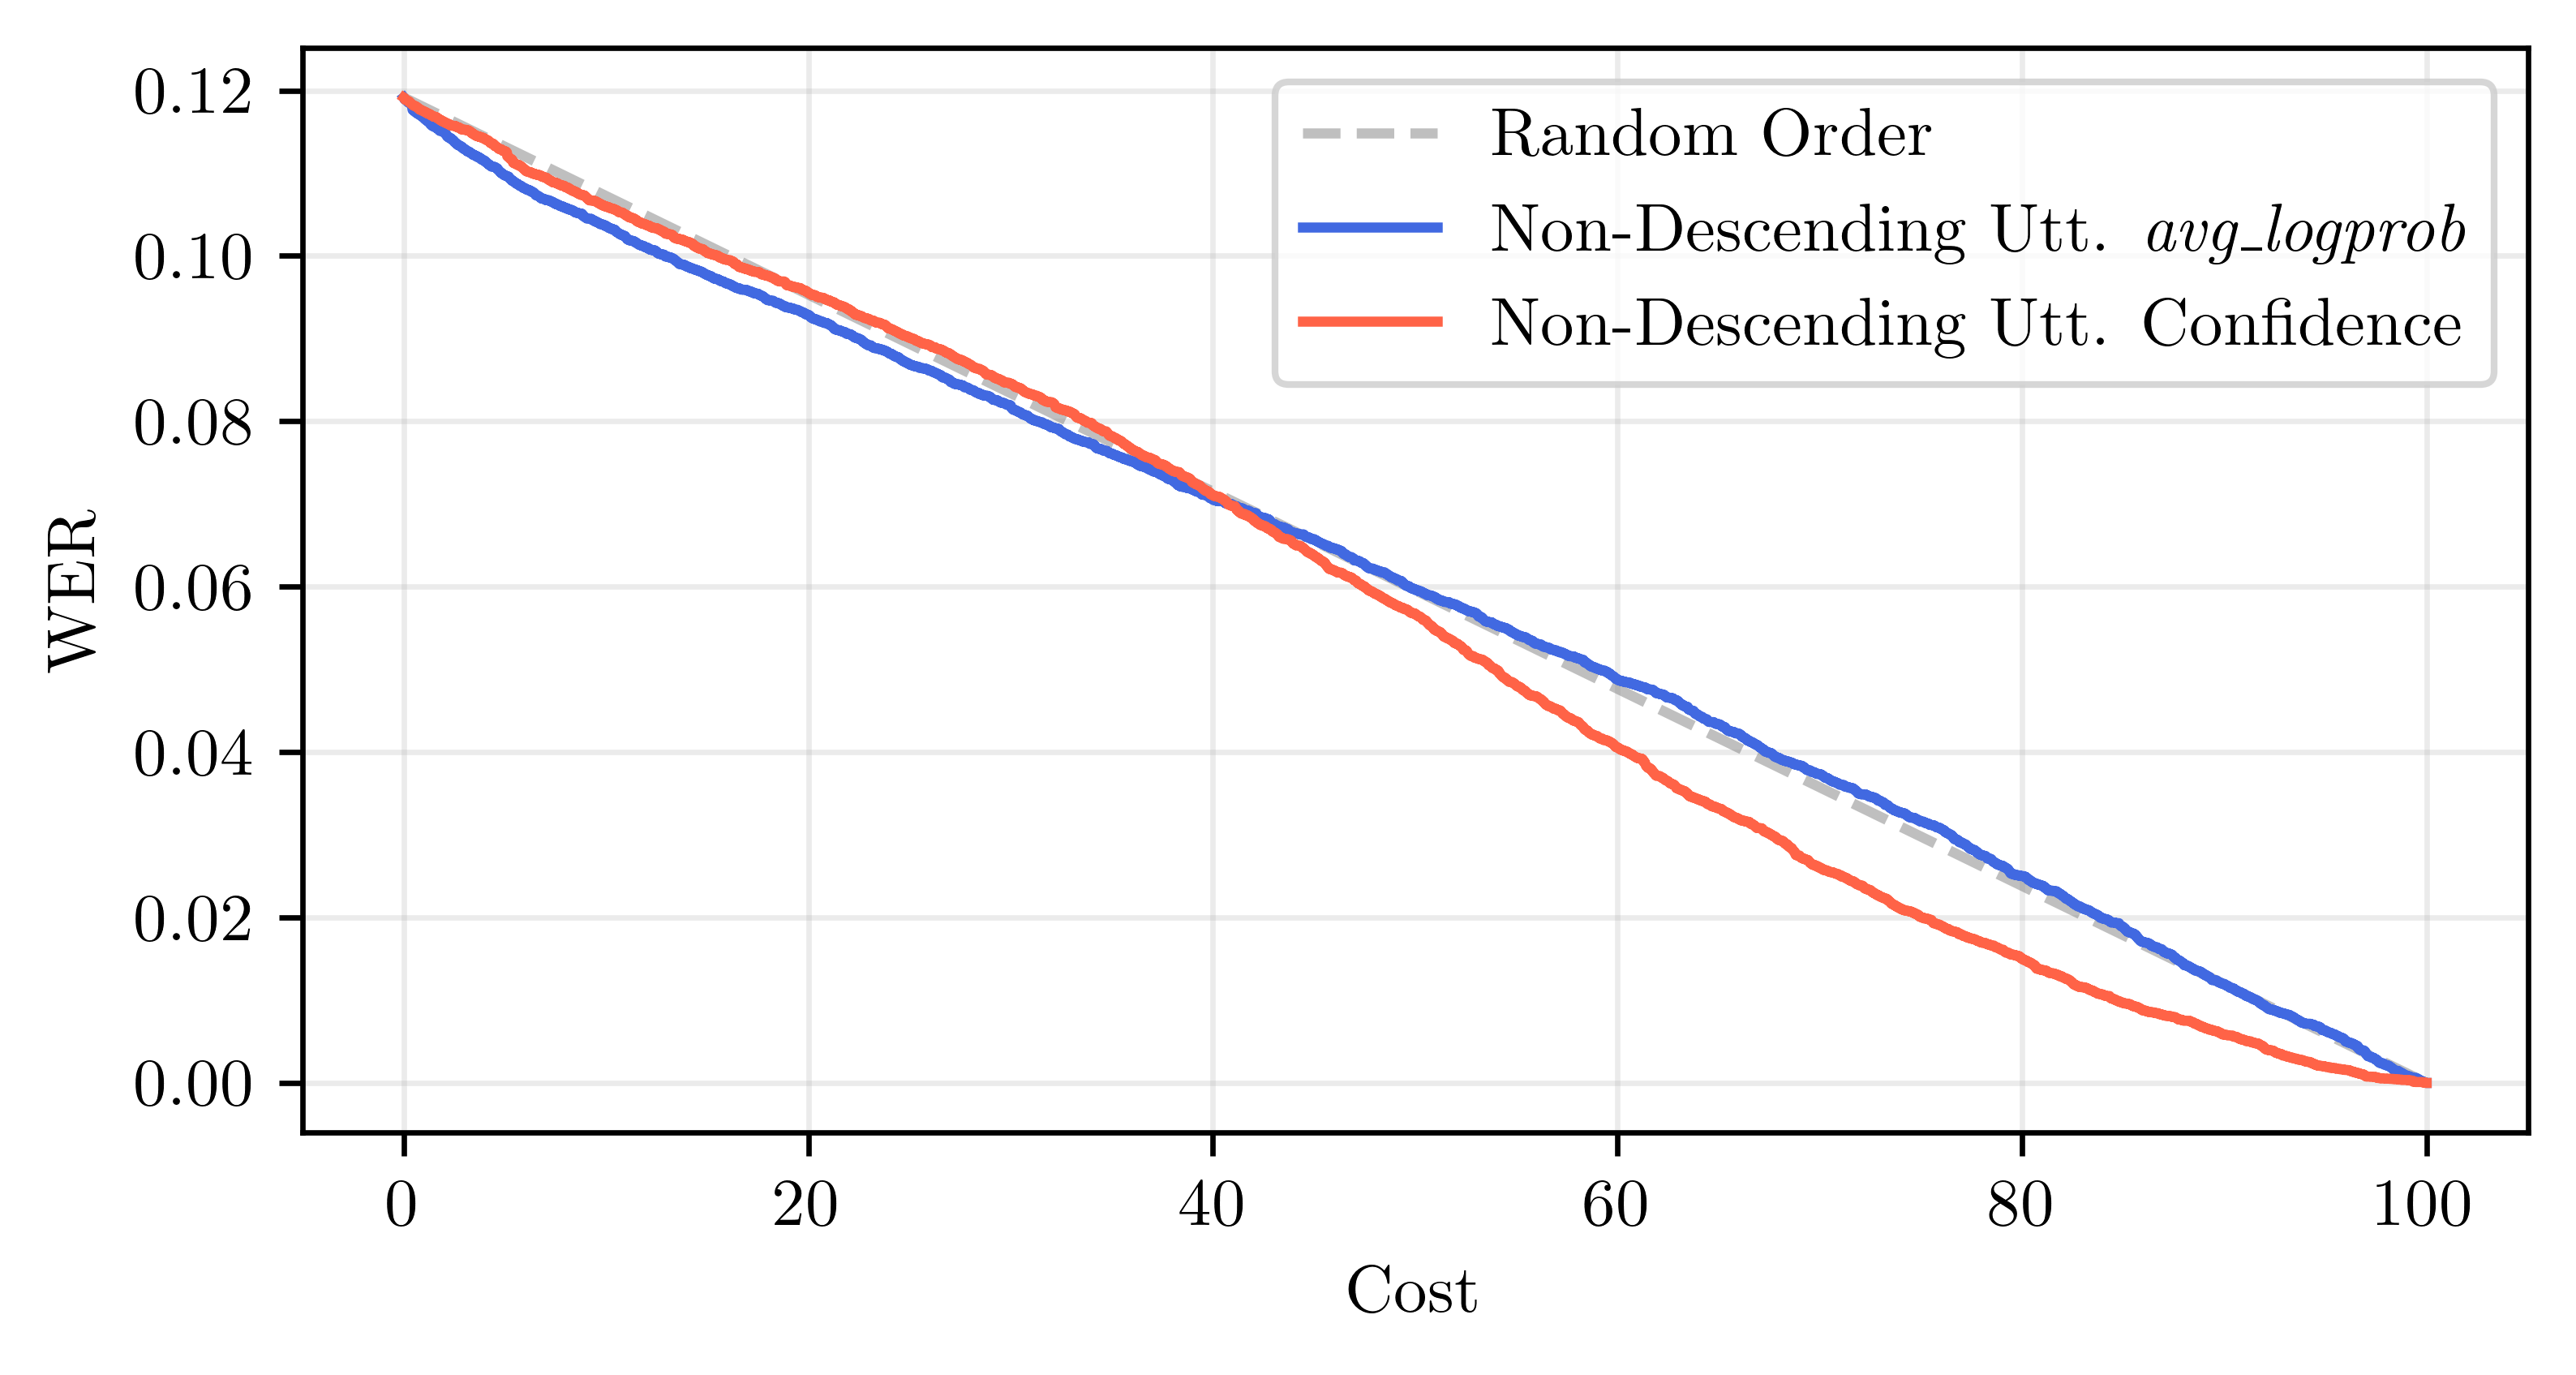
\includegraphics[width=\textwidth]{figures/corpus-avg-lprob-uttconf.png}
 \centering
\end{figure}

\clearpage
\subsection{Per-conversation average results using word-confidence}\label{subsec:avg-word-conf}

\begin{figure}[h!]
 \caption{Ordered by non-descending utterance-minimum word-confidence}
 \label{fig:word-conf-comparison-plot1}
 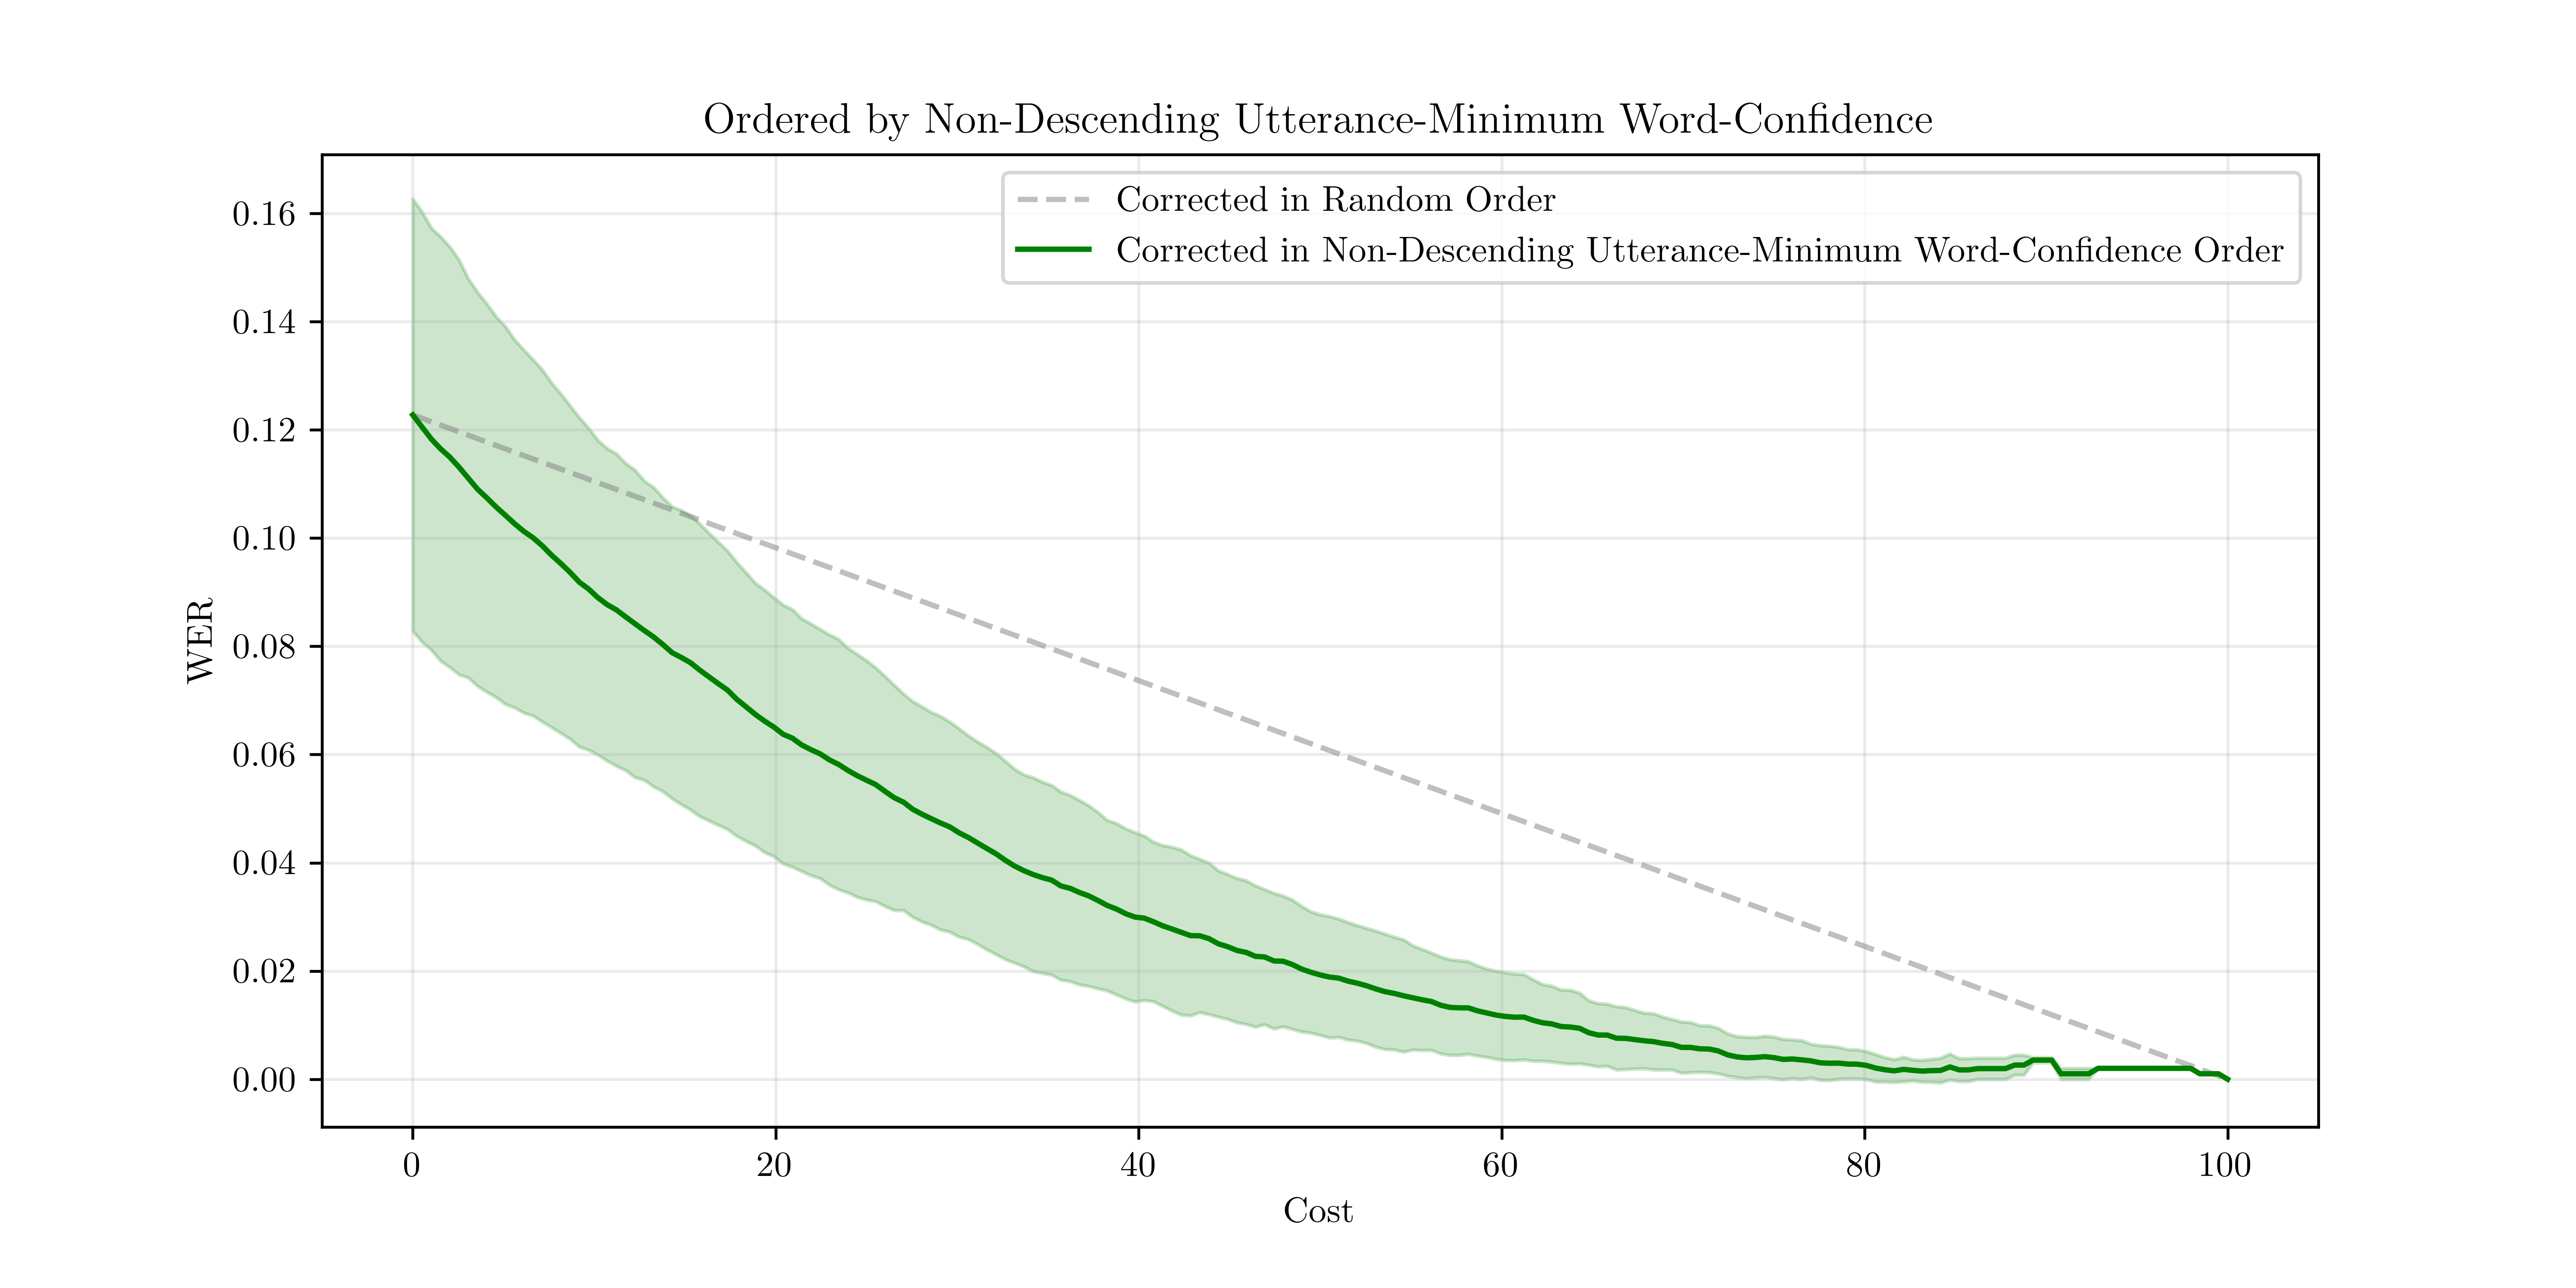
\includegraphics[width=\textwidth]{figures/word-conf-comparison-plot1.png}
 \centering
\end{figure}
\begin{figure}[h!]
 \caption{Ordered by non-ascending utterance-minimum word-confidence}
 \label{fig:word-conf-comparison-plot2}
 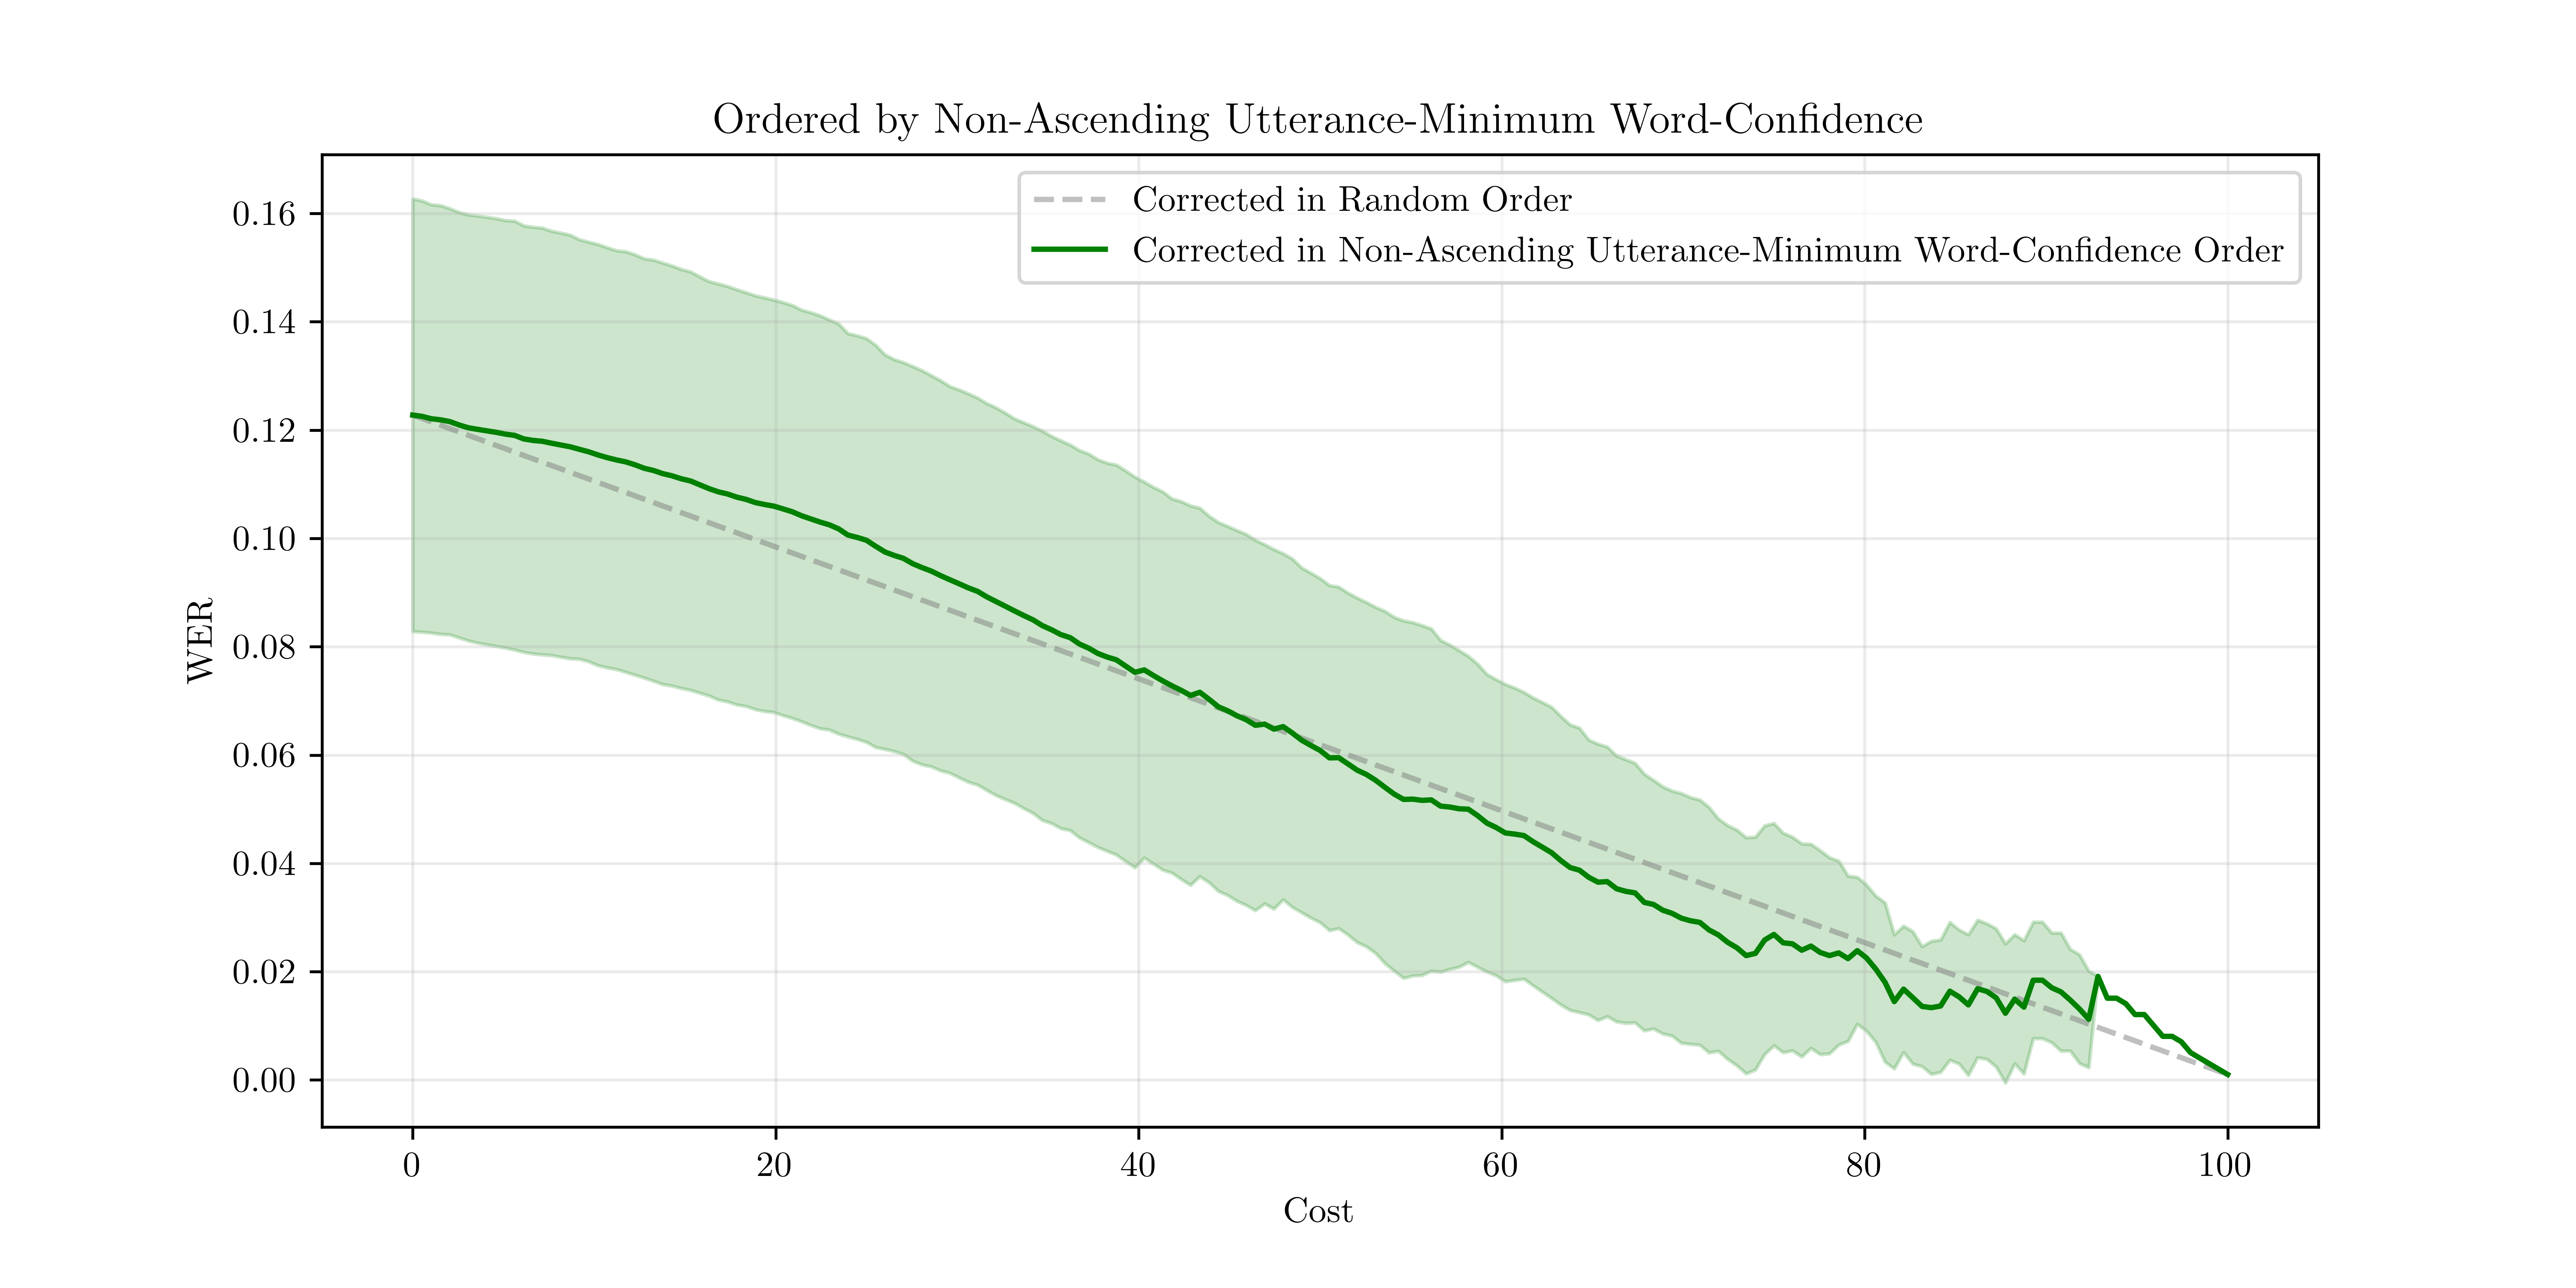
\includegraphics[width=\textwidth]{figures/word-conf-comparison-plot2.png}
 \centering
\end{figure}
\begin{figure}[p]
 \caption{Ordered by non-descending utterance-maximum word-confidence}
 \label{fig:word-conf-comparison-plot3}
 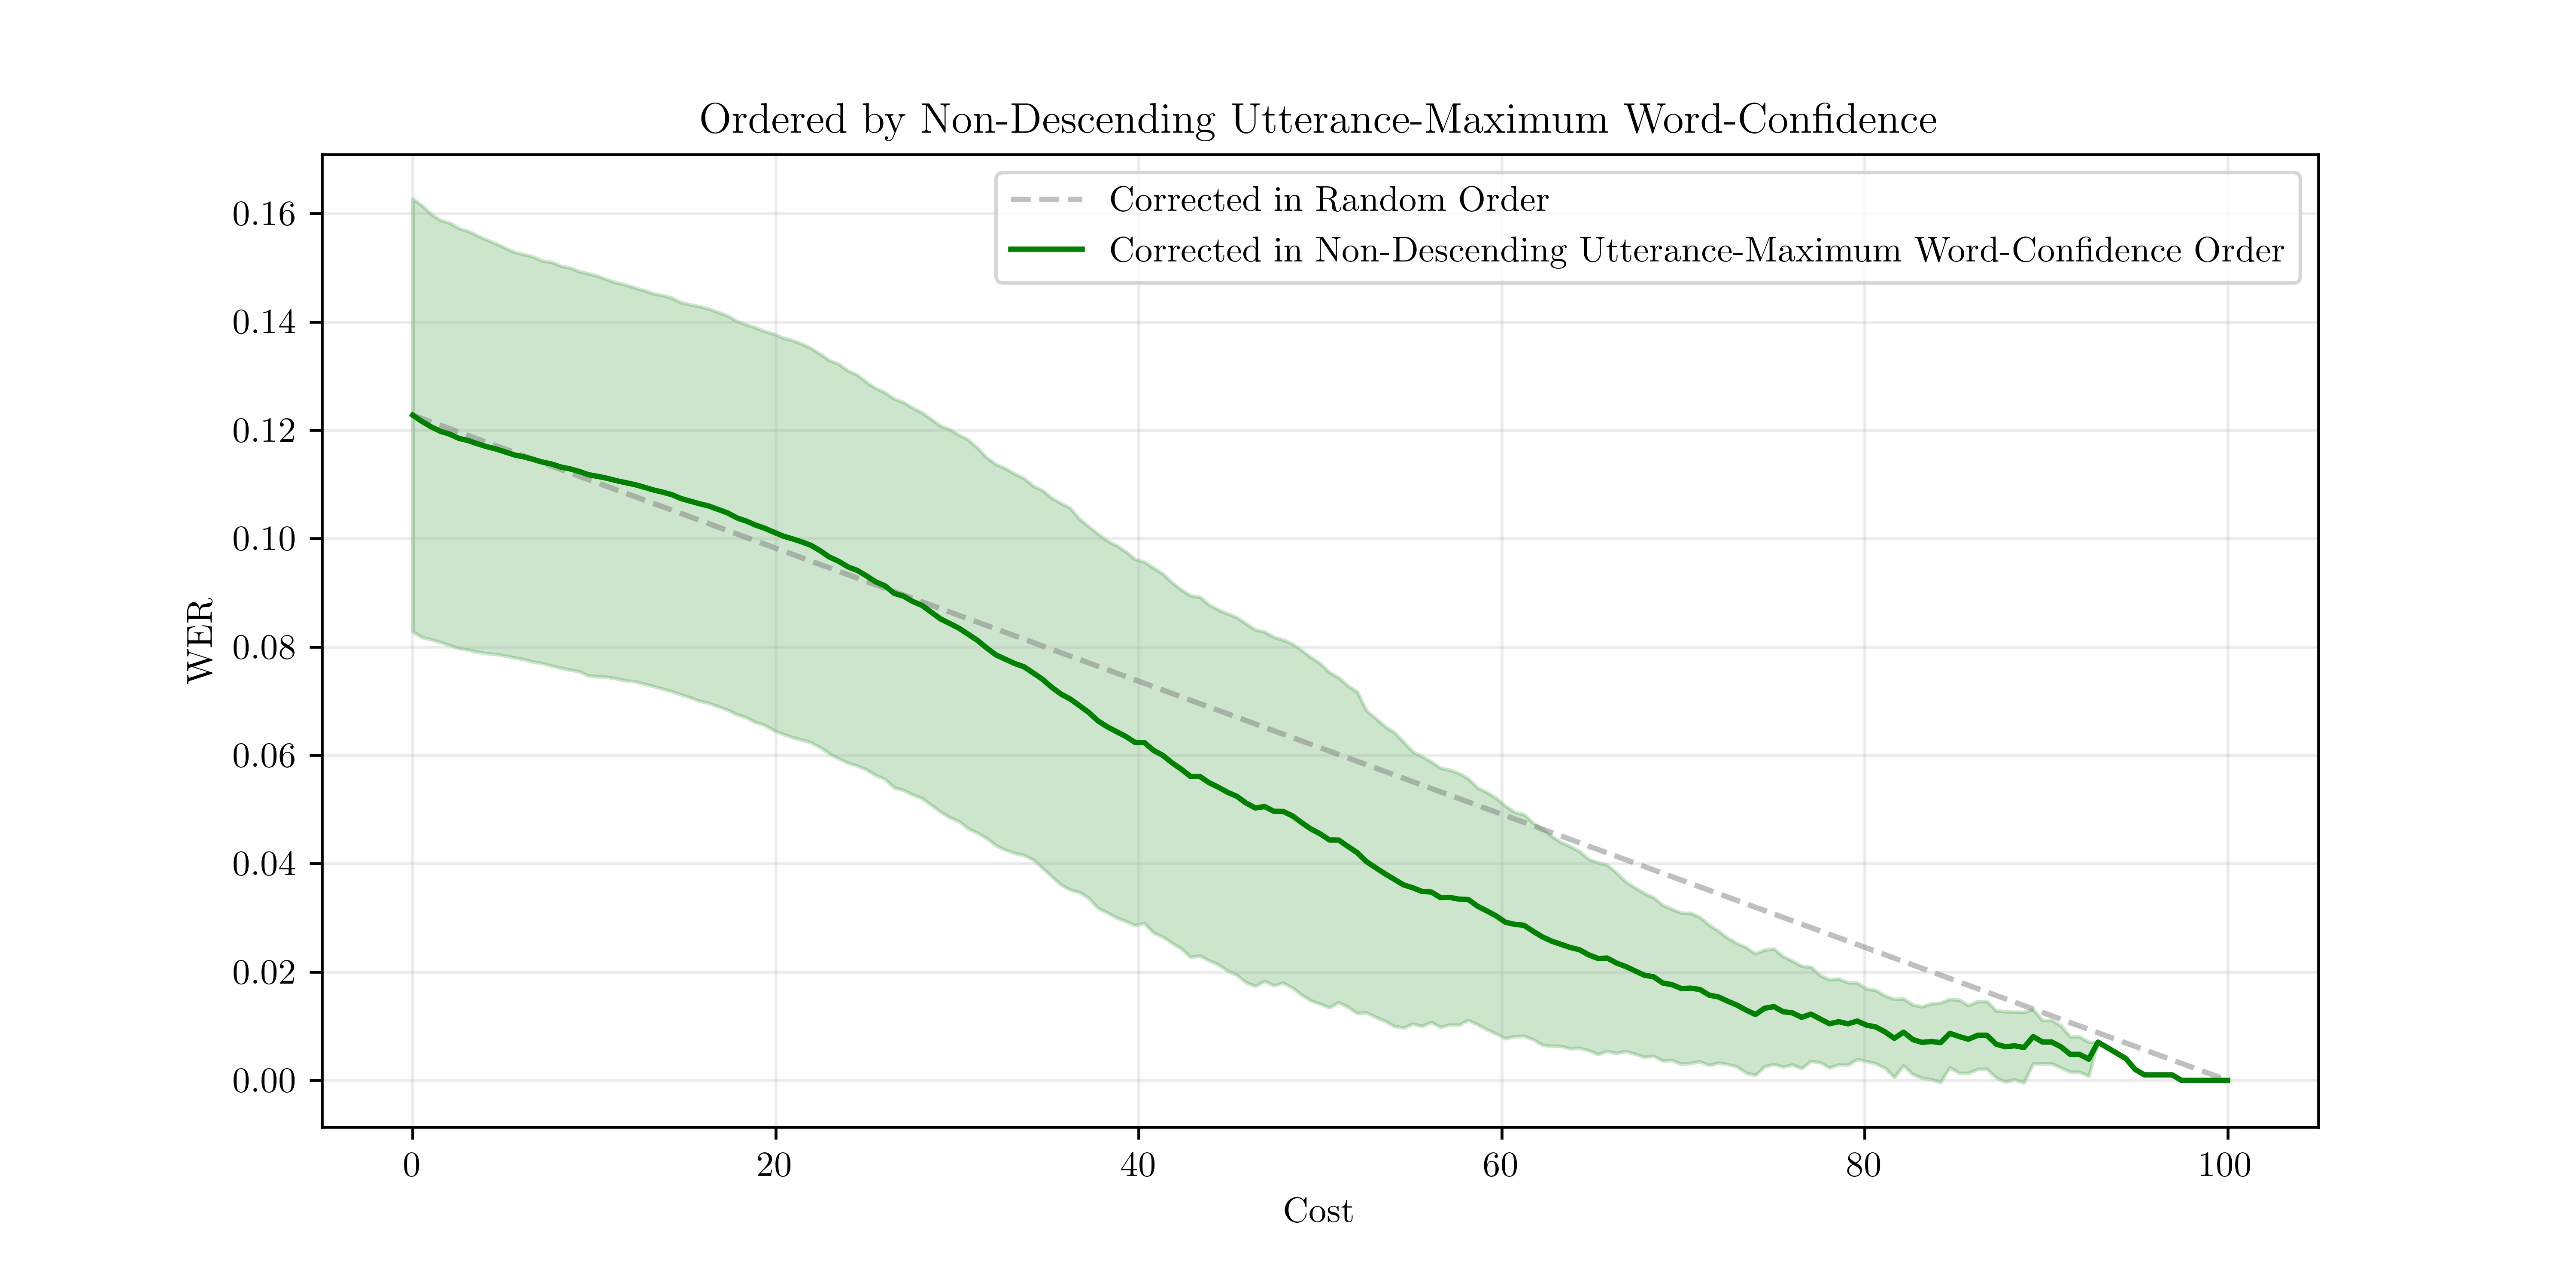
\includegraphics[width=\textwidth]{figures/word-conf-comparison-plot3.png}
 \centering
\end{figure}
\begin{figure}[p]
 \caption{Ordered by non-ascending utterance-maximum word-confidence}
 \label{fig:word-conf-comparison-plot4}
 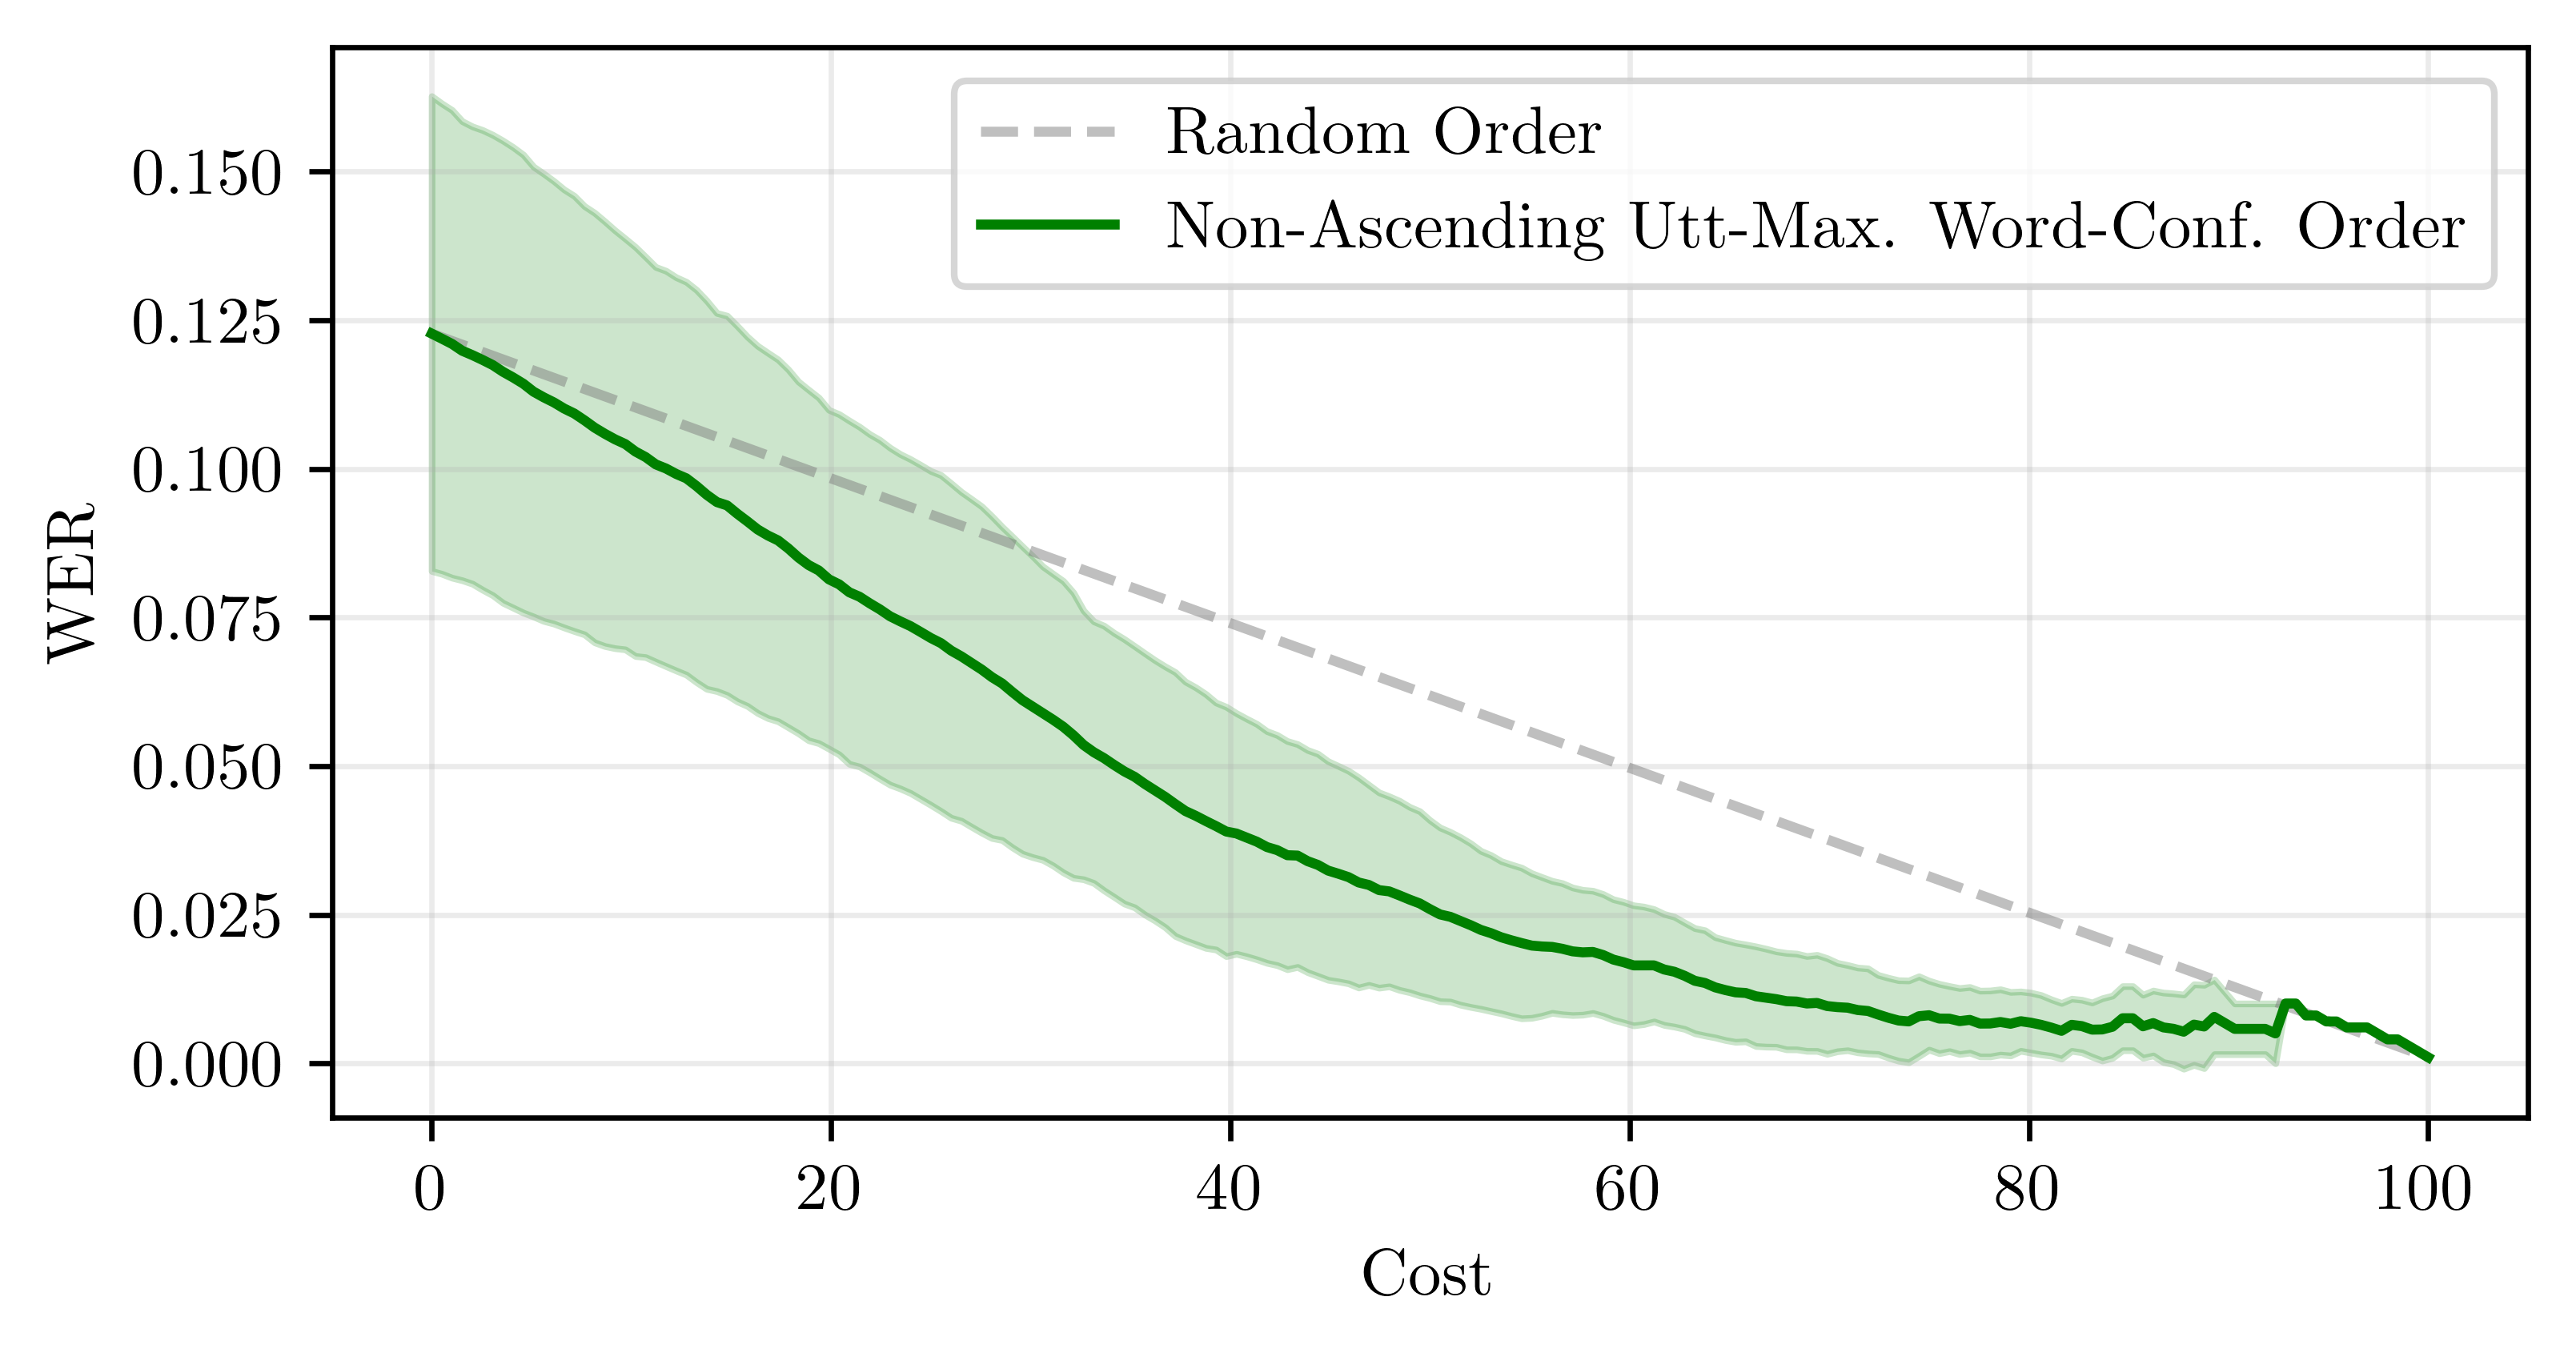
\includegraphics[width=\textwidth]{figures/word-conf-comparison-plot4.png}
 \centering
\end{figure}

\clearpage
\subsection{Corpus-wide comparisons with word-level confidence ordering}\label{subsec:comparing-all}

\begin{figure}[h!]
 \caption{Comparing whole-corpus evaluation performance with each word-confidence ordering}
 \label{fig:corpus-all-word-conf-measures}
 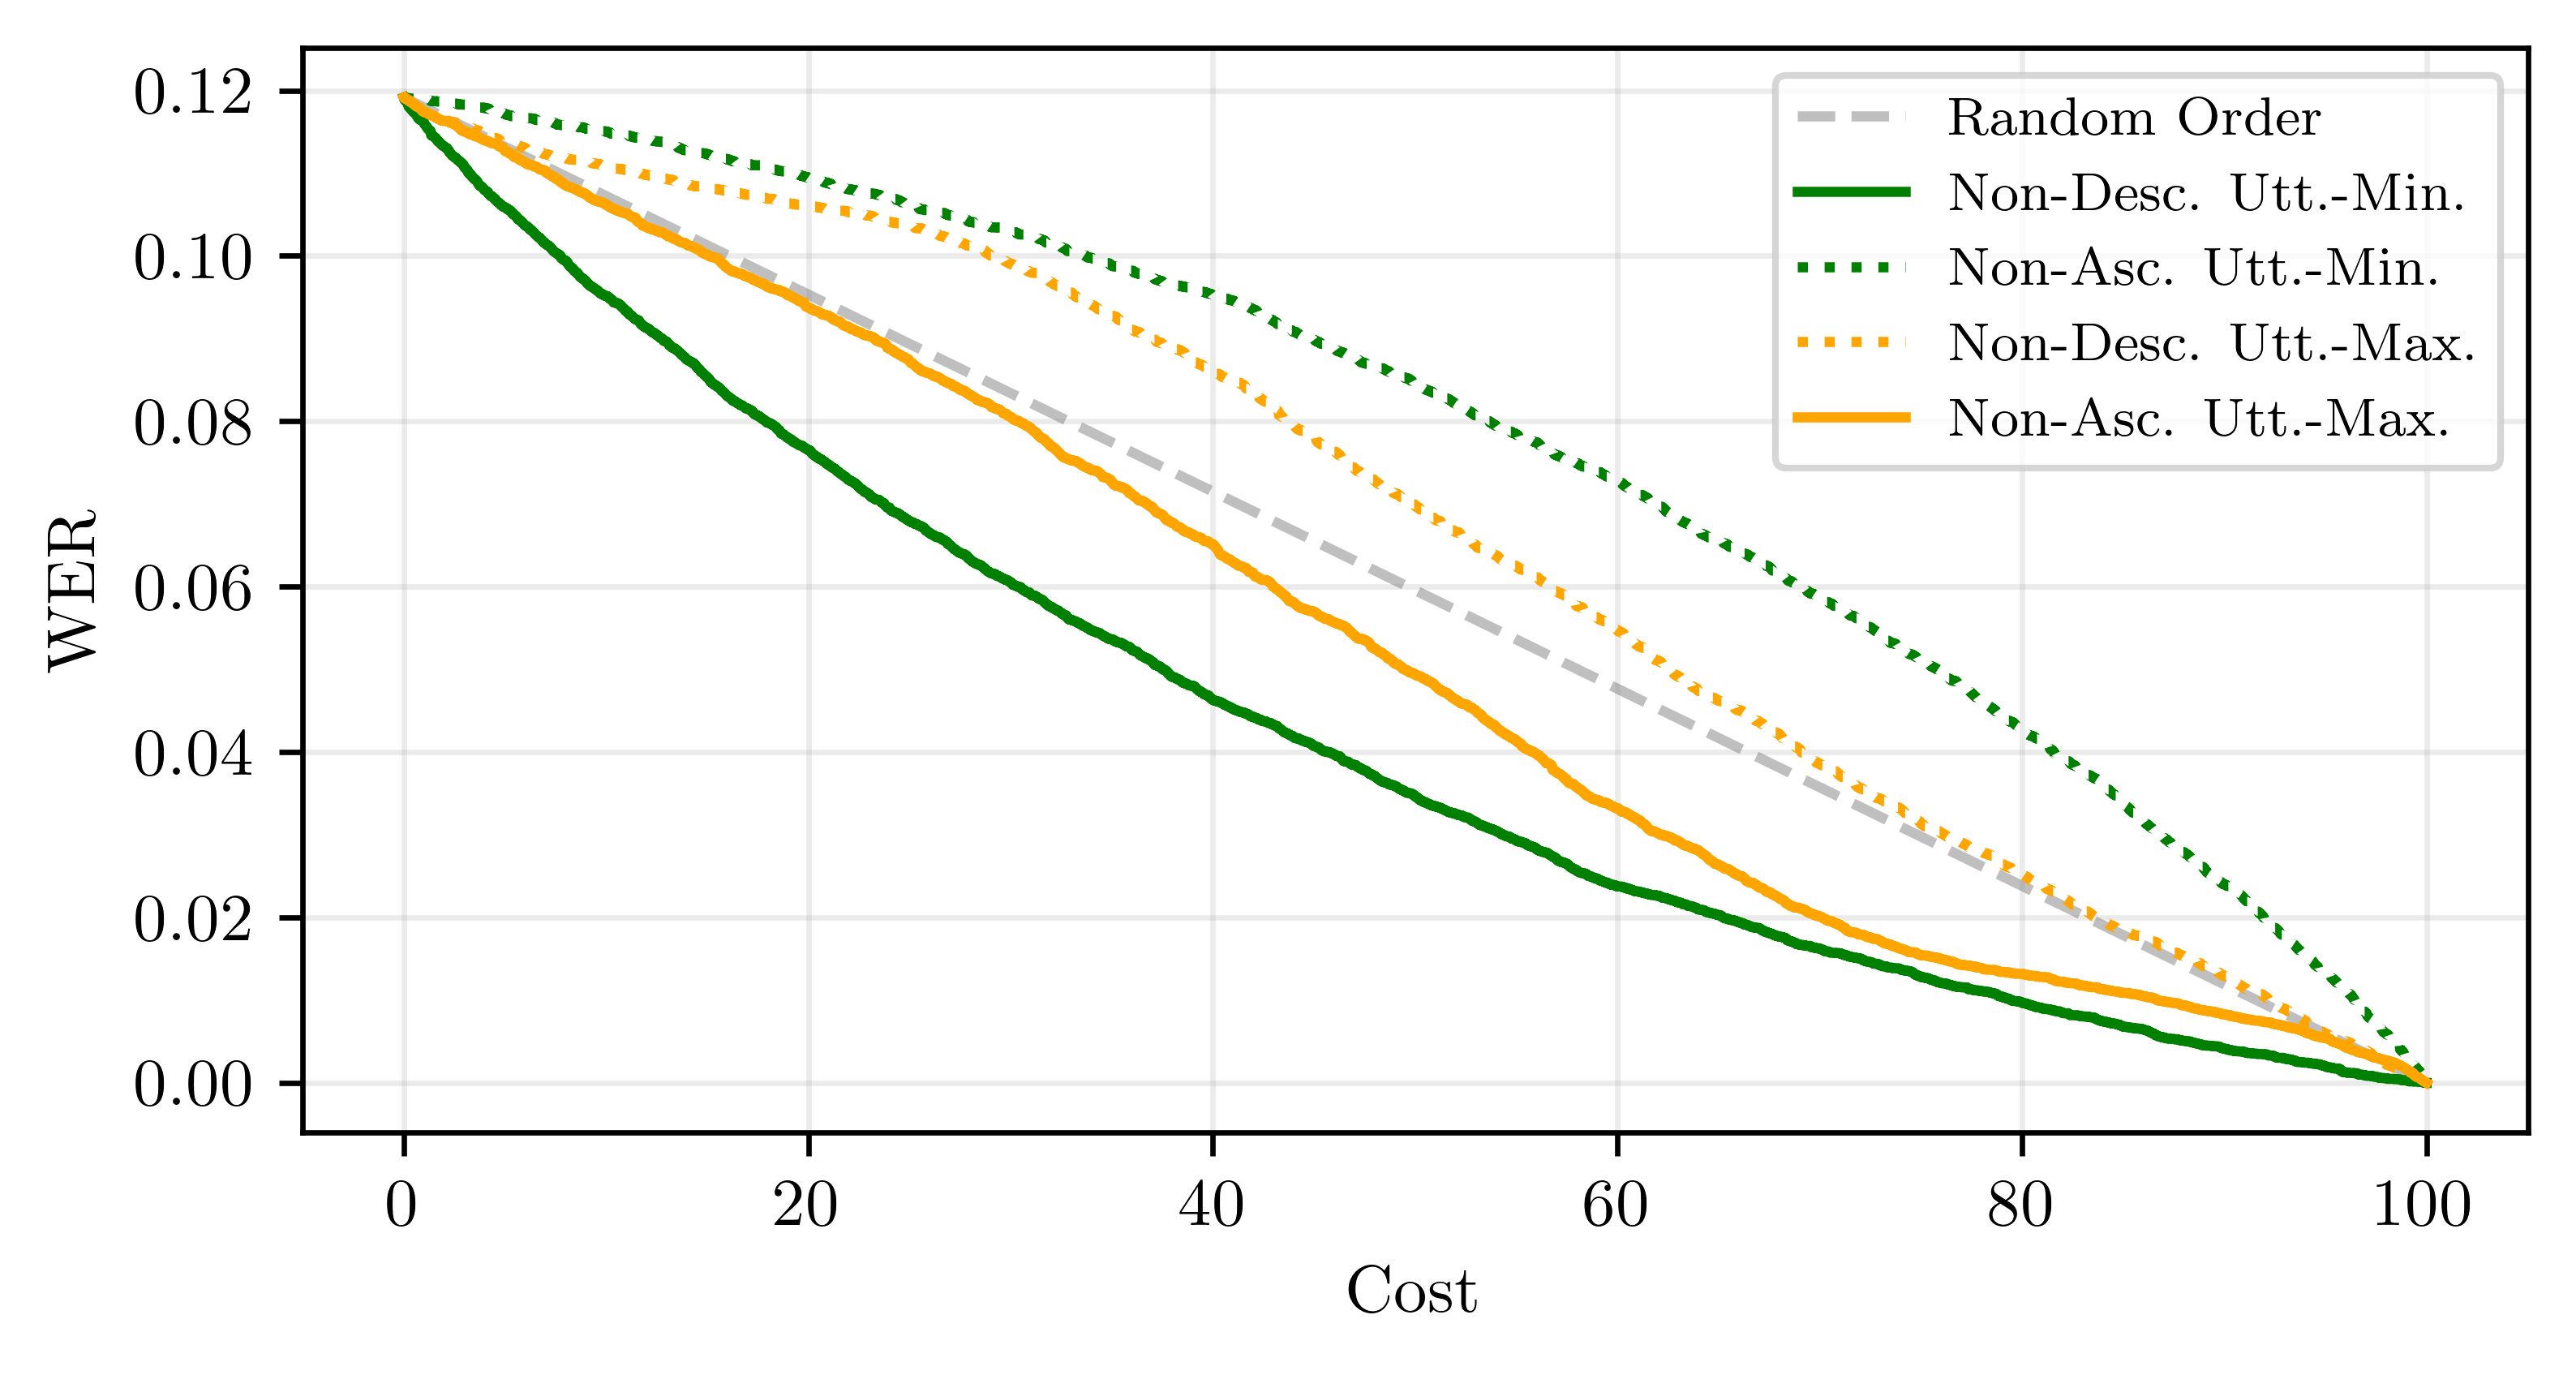
\includegraphics[width=\textwidth]{figures/corpus-all-word-conf-measures.png}
 \centering
\end{figure}
\begin{figure}[h!]
 \caption{Comparing whole-corpus evaluation performance with each ordering metric}
 \label{fig:corpus-allmeasures}
 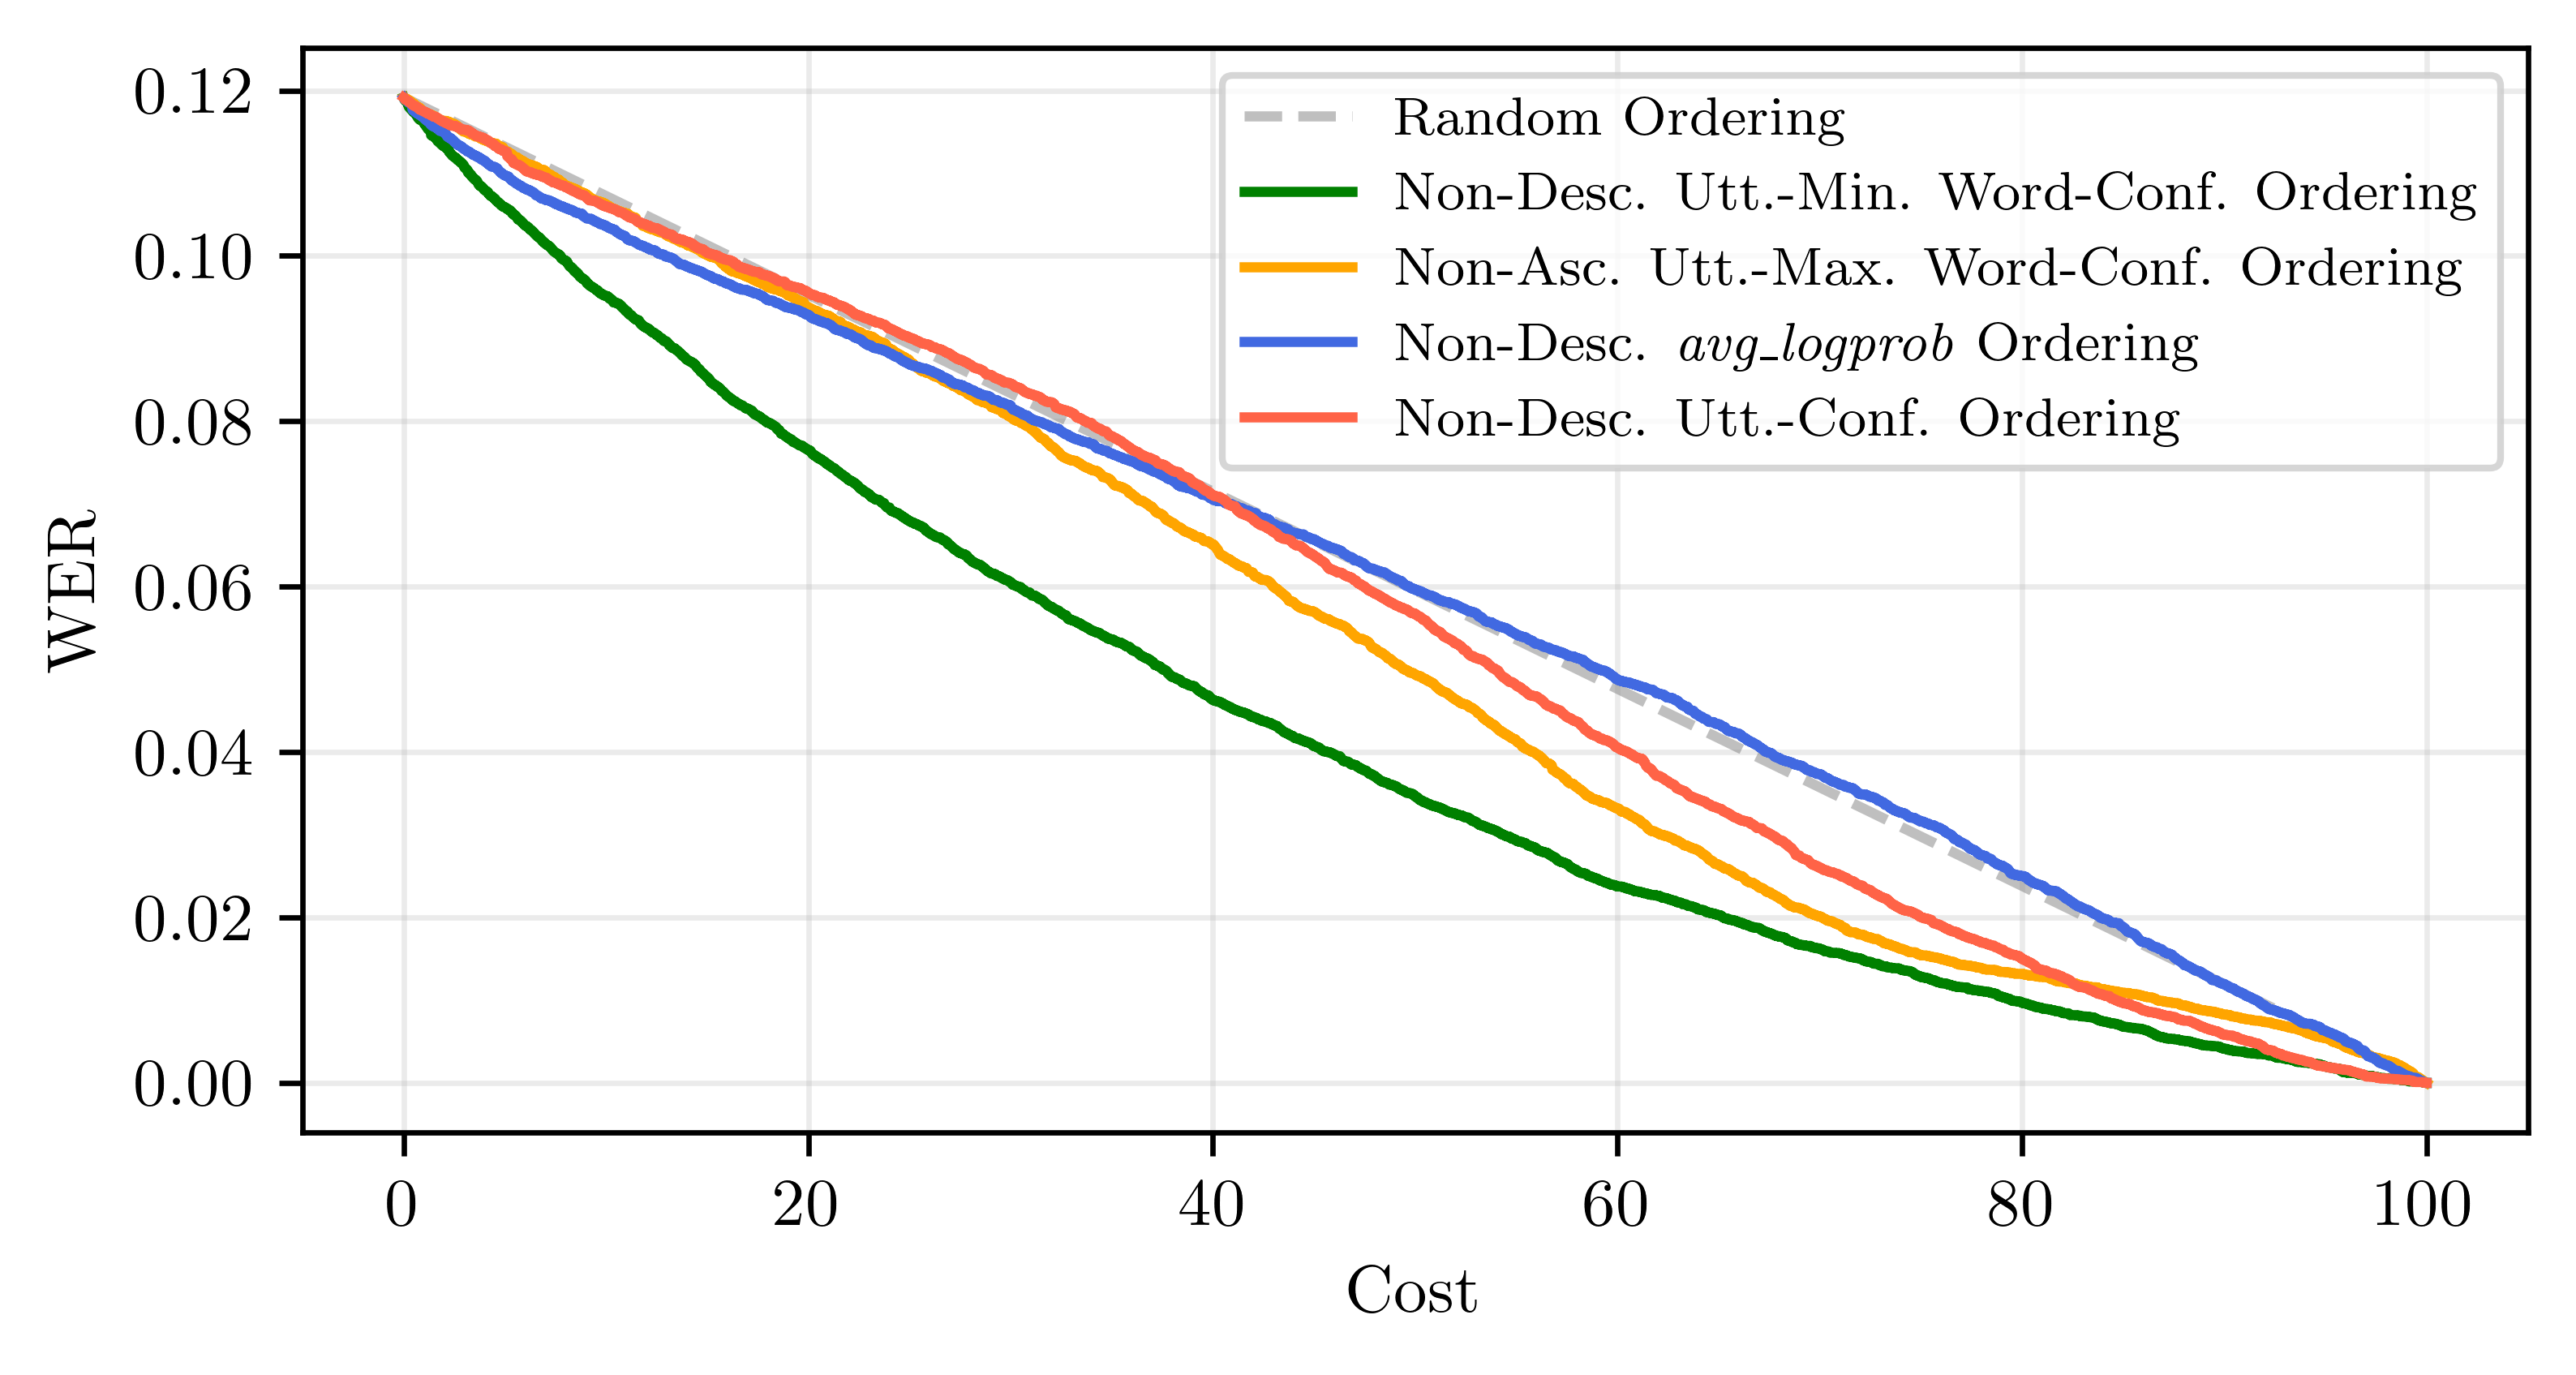
\includegraphics[width=\textwidth]{figures/corpus-allmeasures.png}
 \centering
\end{figure}

\clearpage
\subsection{Different word-level confidence scoring techniques}\label{subsec:more-techniques}

\begin{figure}[h!]
 \caption{Comparing whole-corpus evaluation performance with different word-level confidence metrics}
 \label{fig:range-ordering-vs-stddev-vs-min-wconf}
 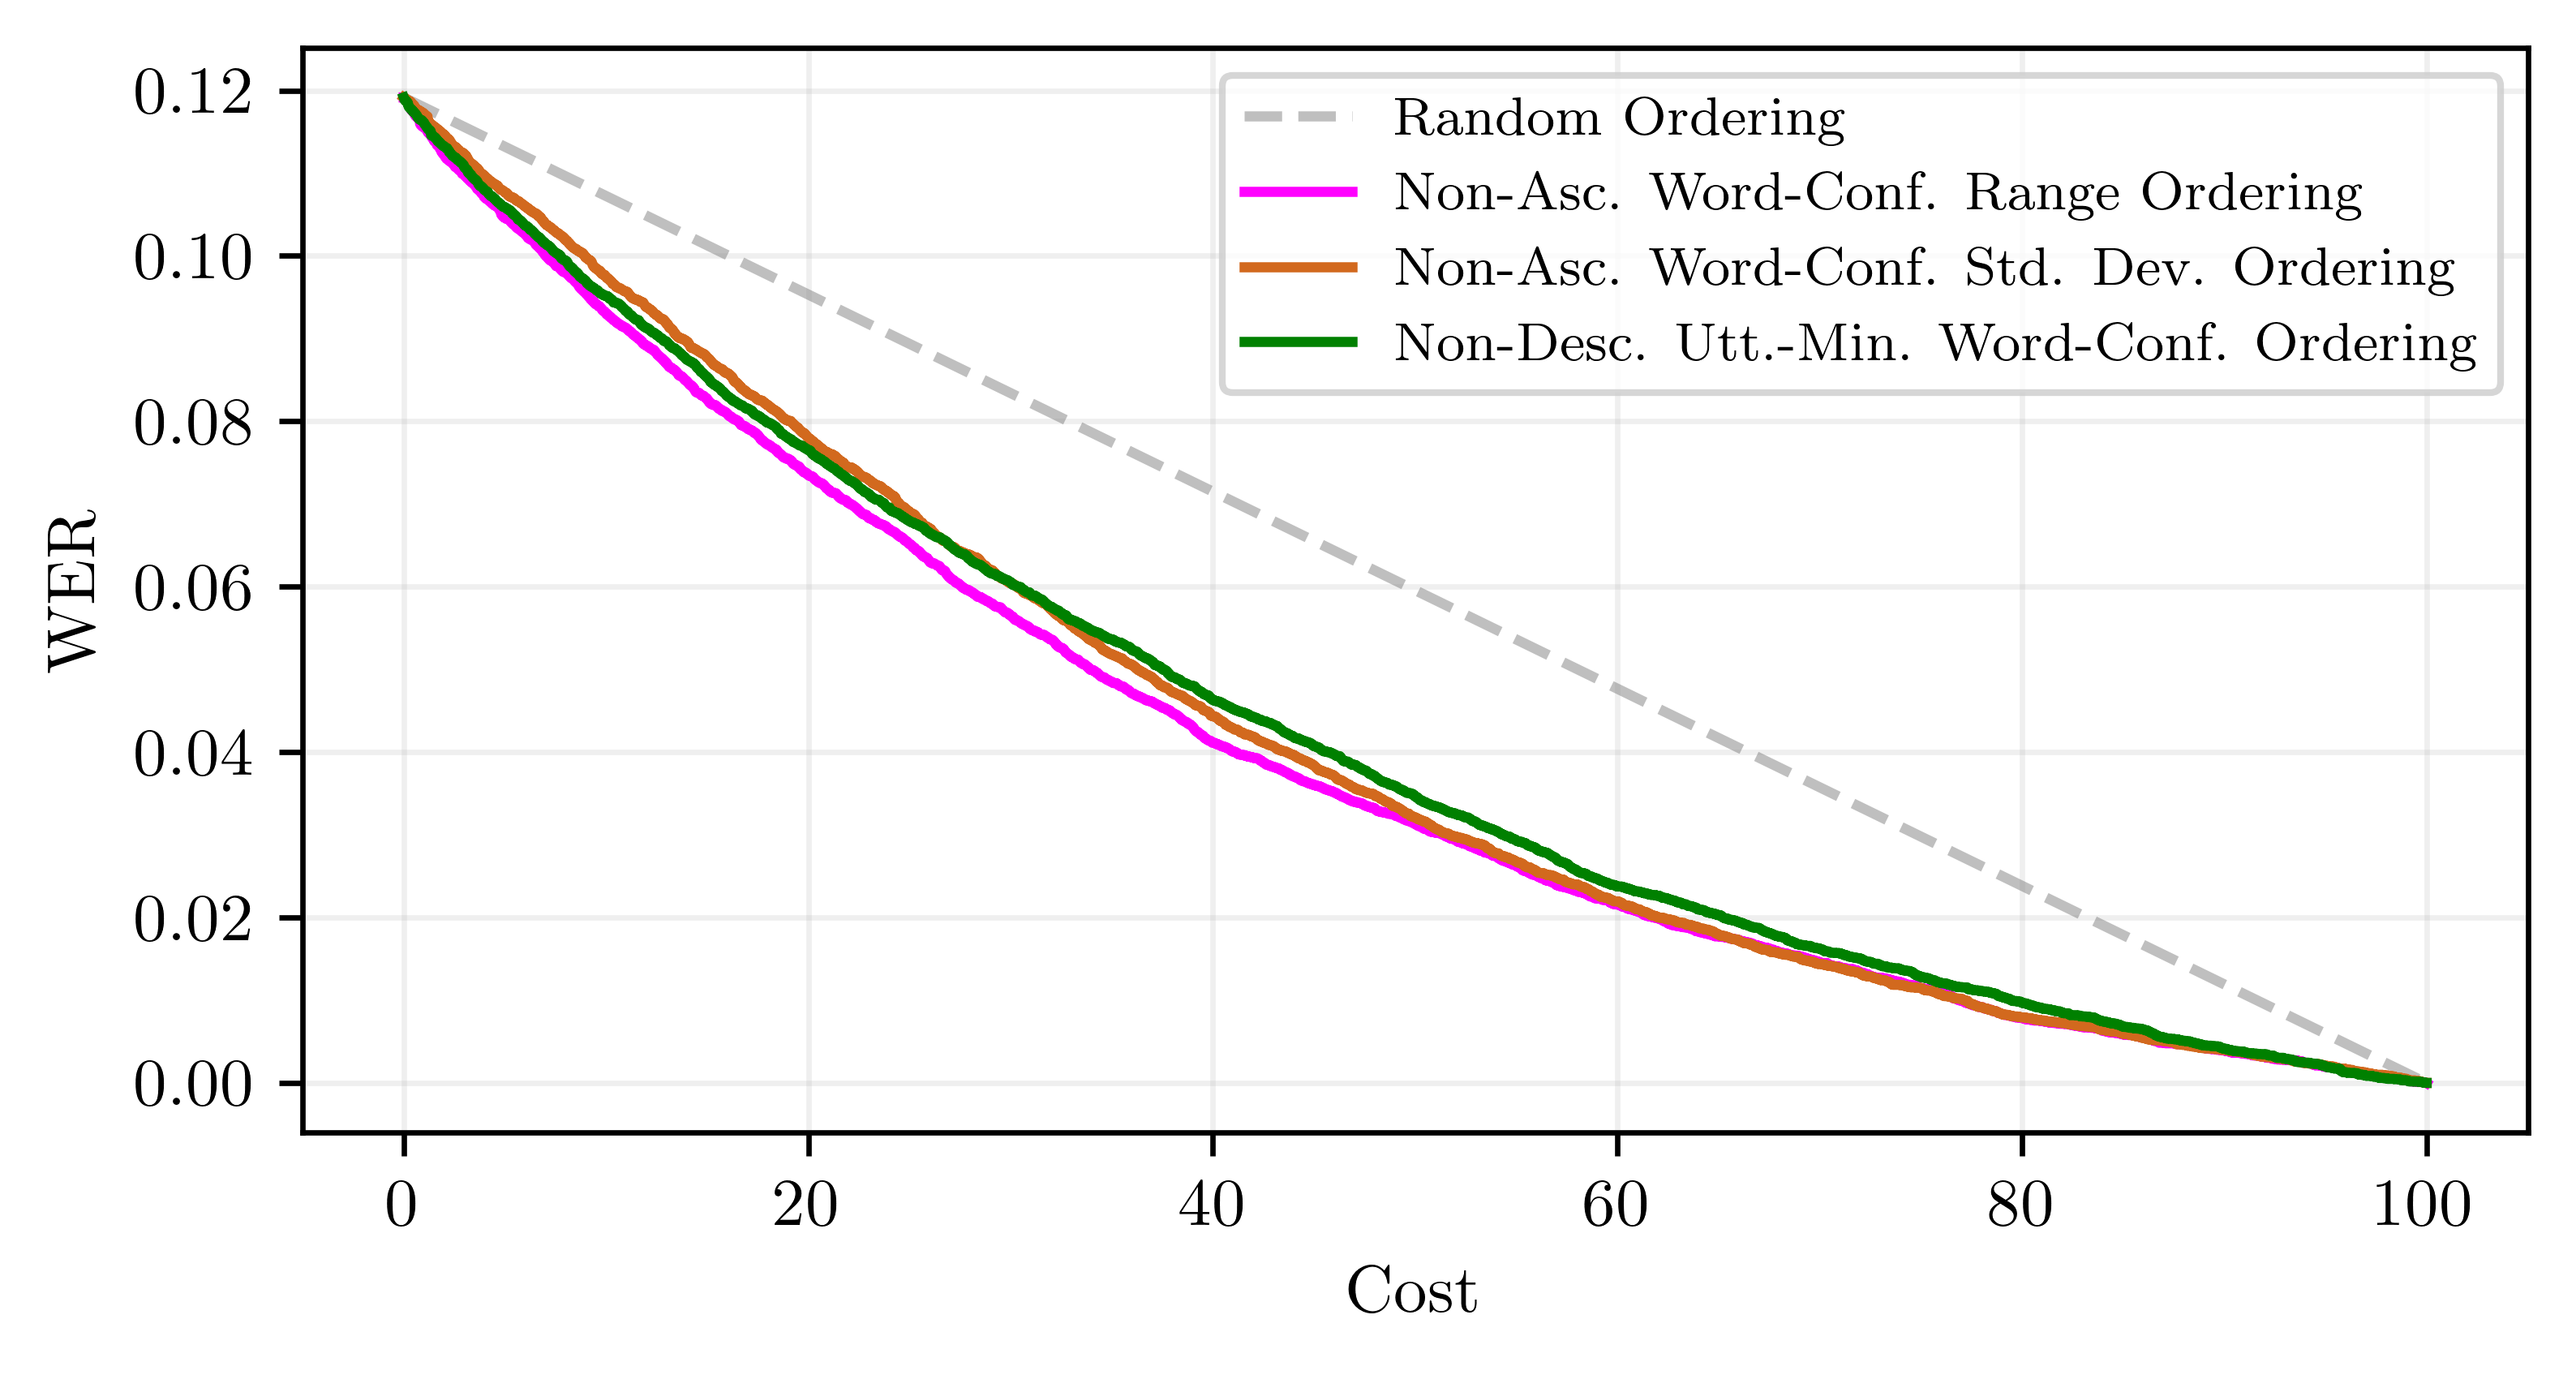
\includegraphics[width=\textwidth]{figures/range-ordering-vs-stddev-vs-min-wconf.png}
 \centering
\end{figure}
\begin{figure}[h!]
 \caption{WER difference between metrics and random ordering}
 \label{fig:delta-wer}
 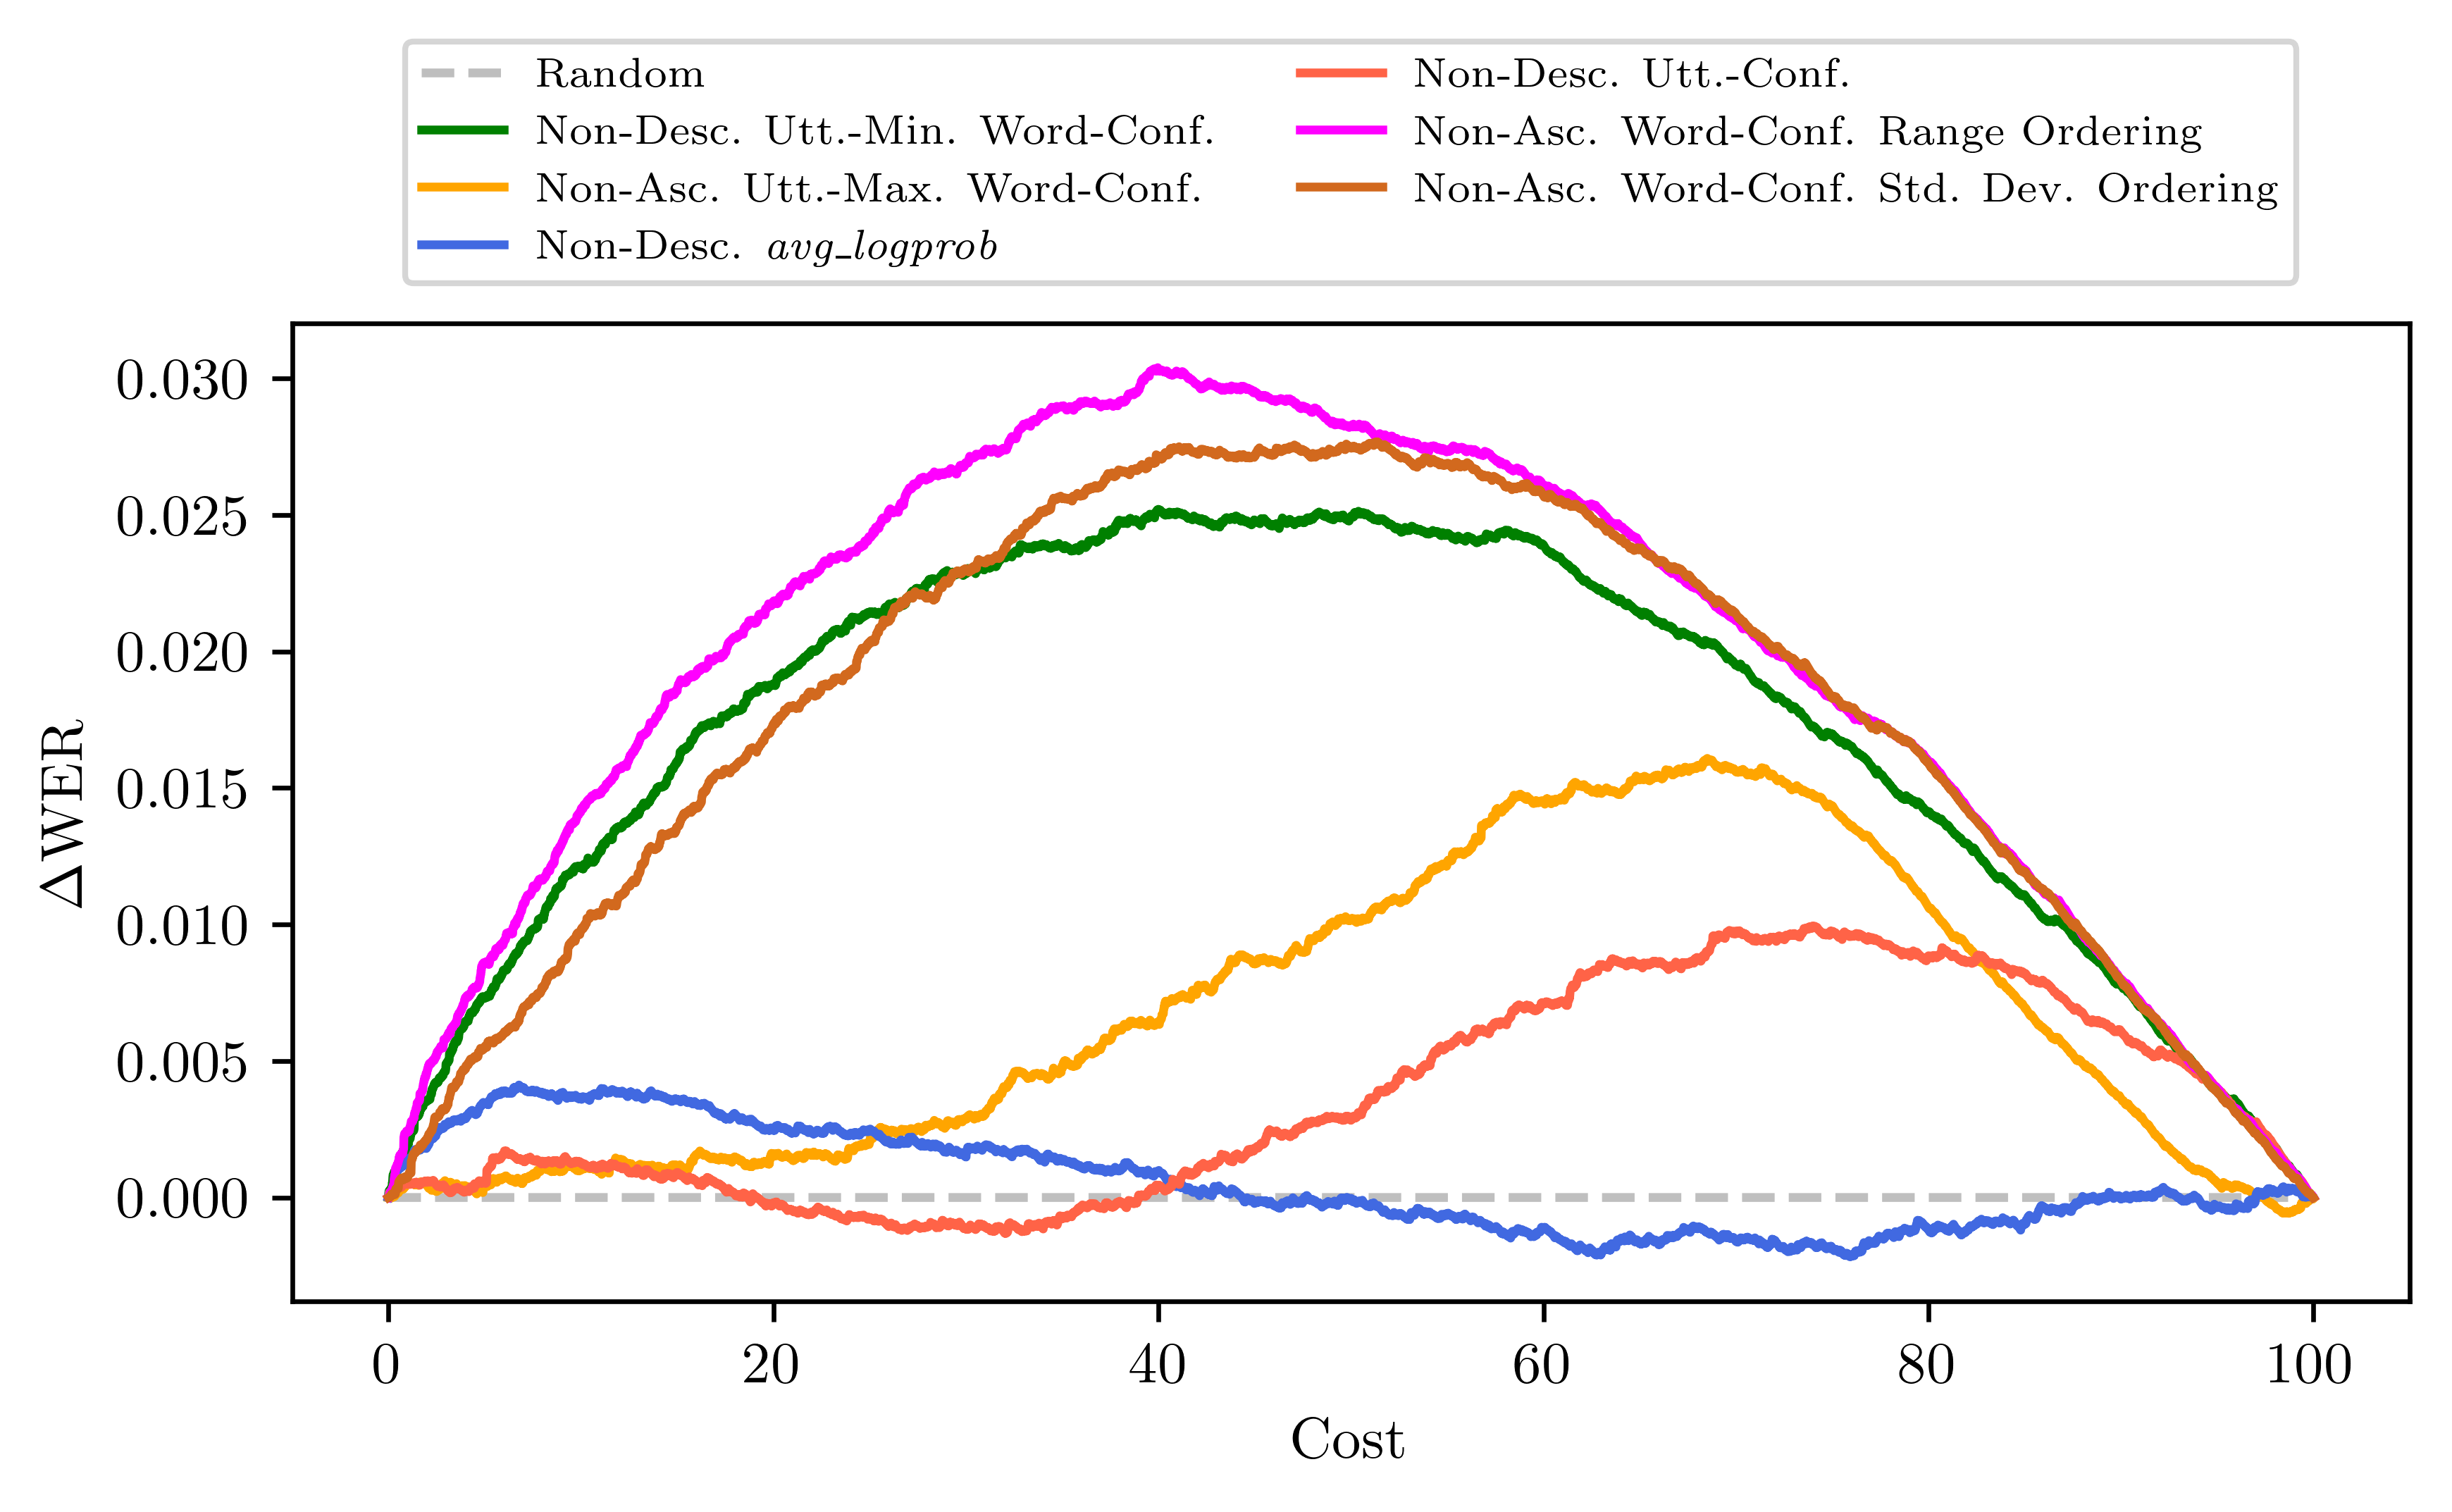
\includegraphics[width=\textwidth]{figures/delta-wer-all-allmeasures.png}
 \centering
\end{figure}


